\documentclass{jarticle}
\usepackage{robomech}
\usepackage{graphicx}
\usepackage{amsmath}
\usepackage{bm}
\usepackage{here}
\usepackage{siunitx}
\usepackage{subcaption}

\begin{document}
\makeatletter
\title{飛行ロボットによるパーチングと物体把持を両立可能にするトライフォース・ハンドの設計と機体制御}
{Design and control of the tri-force hand for perching and object grasping with aerial robots}
% {―日本語副題:ゴシック体・12pt(欧文Arial・12pt)―}
{}
{}
% {-English Subtitle: Times New Roman, 10pt-}

\author{
\begin{tabular}{ll}
 \hspace{1zw}○ 学\hspace{1zw}飯田央明 (東京大)& 正\hspace{1zw} 趙漠居(東京大) \\ \hspace{1zw} 杉原淳一朗(東京大)& \hspace{1zw} 杉原和輝(東京大) \\ \hspace{1zw} 小塚陽希(東京大)& \hspace{1zw} 李謹傑(東京大) \\ \hspace{1zw} 長藤圭介(東京大)& \hspace{1zw}
%  \hspace{1zw}学\hspace{1zw}東京 学(西大)& [日本語著者名:明朝体10pt]\\
 % ※協賛・後援団体の会員資格で発表される場合は「正・学」は不要です。
 \end{tabular}
 % &\\
 \vspace{1zh} \\
 \begin{tabular}{l}
{\small Hisaaki IIDA, University of Tokyo, iida@dragon.t.u-tokyo.ac.jp}\\
 {\small Moju ZHAO, University of Tokyo, }\\
 {\small Junichiro SUGIHARA, University of Tokyo,}
 ~{\small Kazuki SUGIHARA, University of Tokyo}\\
 {\small Haruki KOZUKA, University of Tokyo,}
 ~{\small Jinjie LI, University of Tokyo}\\
 {\small Keisuke NAGATO, University of Tokyo,}\\
\end{tabular}
}
\makeatother

\abstract{ \small 
Recently, as the expectations for aerial robots to perform complex tasks increase, perching has been studied as a method to reduce power consumption during stationary phases by enabling the robot to attach to environmental objects, thereby extending the operational time of power-intensive aerial robots.
However, many existing approaches mount the attachment mechanism on the top or bottom of the robot, which severely restricts the attachment direction and flight posture to prevent the robot from tipping over or coming into contact with the environment and objects.
Additionally, many of these robots are designed specifically for perching and cannot perform other tasks.  
To address these issues simultaneously, we propose the development of an end-effector capable of both lateral perching and grasping a variety of objects and tools.
However, no previous research has successfully achieved both stable lateral perching and precise object grasping using a rotorcraft. Furthermore, implementing perching and transitioning back to flight in this study requires specialized flight control techniques.  
Therefore, this study aims to design a three-fingered tendon-driven hand powered by a single actuator as an end-effector capable of stable multi-directional perching and precise object grasping. Additionally, we will develop the motion planning for an aerial robot equipped with this hand.
}

\date{} % 日付を出力しない
\keywords{aerial robot, mechanical hand, tendon driven, perching, grasping}

\maketitle
\thispagestyle{empty}
\pagestyle{empty}

\small
\section{序論}
これまで、制約の少ない空路を利用した物体搬送や工場設備等の監視業務用インフラとして飛行ロボットを利用する企業や研究が現れ、飛行ロボットの社会進出が進んできた。近年、飛行ロボットに期待される役割はより複雑化し、飛行ロボットが単体で実行する空撮などのタスクから、外部の物体や環境との物理接触を含む高度な作業へ移行している。特に高所での作業や電線工事など、人間の作業員が行っていた危険作業を飛行ロボットに代替させる事例が増えている。複雑タスクの実行可能化に関して、複数の劣駆動機体による協調作業を扱った研究が行われている。しかし複数機体間での連携は単一機体の場合に比べて困難かつ不安定であり、機体の導入にも多くのコストがかかるという問題がある。自由度が高い全駆動機体を用いた研究も行われているが、飛行や作業に伴って消費する電力量が大きくなるため、長時間の駆動が難しくなるという問題がある。そこで本研究では、全駆動飛行ロボットの安定した機体制御性と単一機体での複数タスク実行能力を両立しつつ、消費電力を低減させることで長時間駆動を可能にすることを目指す。

消費電力の低減に関して、環境物体に結合し自重を支持することでロータの推力を用いず空中に留まるパーチングが研究されている。現状では機体の上部または下部にハンド機構を持つものが多くを占めるが、結合目標位置周辺に突出部や壁面が存在する場合では機体が環境物体と接触するリスクがあるため、両者ともに結合時のアプローチ方向や結合位置の制限を強く受ける。一方、固定翼型飛行ロボットにおいては横方向からの結合アプローチに関する研究例がある。このようなパーチングは特に壁面への結合過程において、前述した機体と環境物体との接触リスクを低減可能であるが、固定翼型飛行ロボットは回転翼式飛行ロボットに比べて空中定位可能性や姿勢制御性に欠けるため、タスク実行能力が低い。
\begin{figure}[tb]
  \centering
  \begin{subfigure}{0.25\columnwidth}
    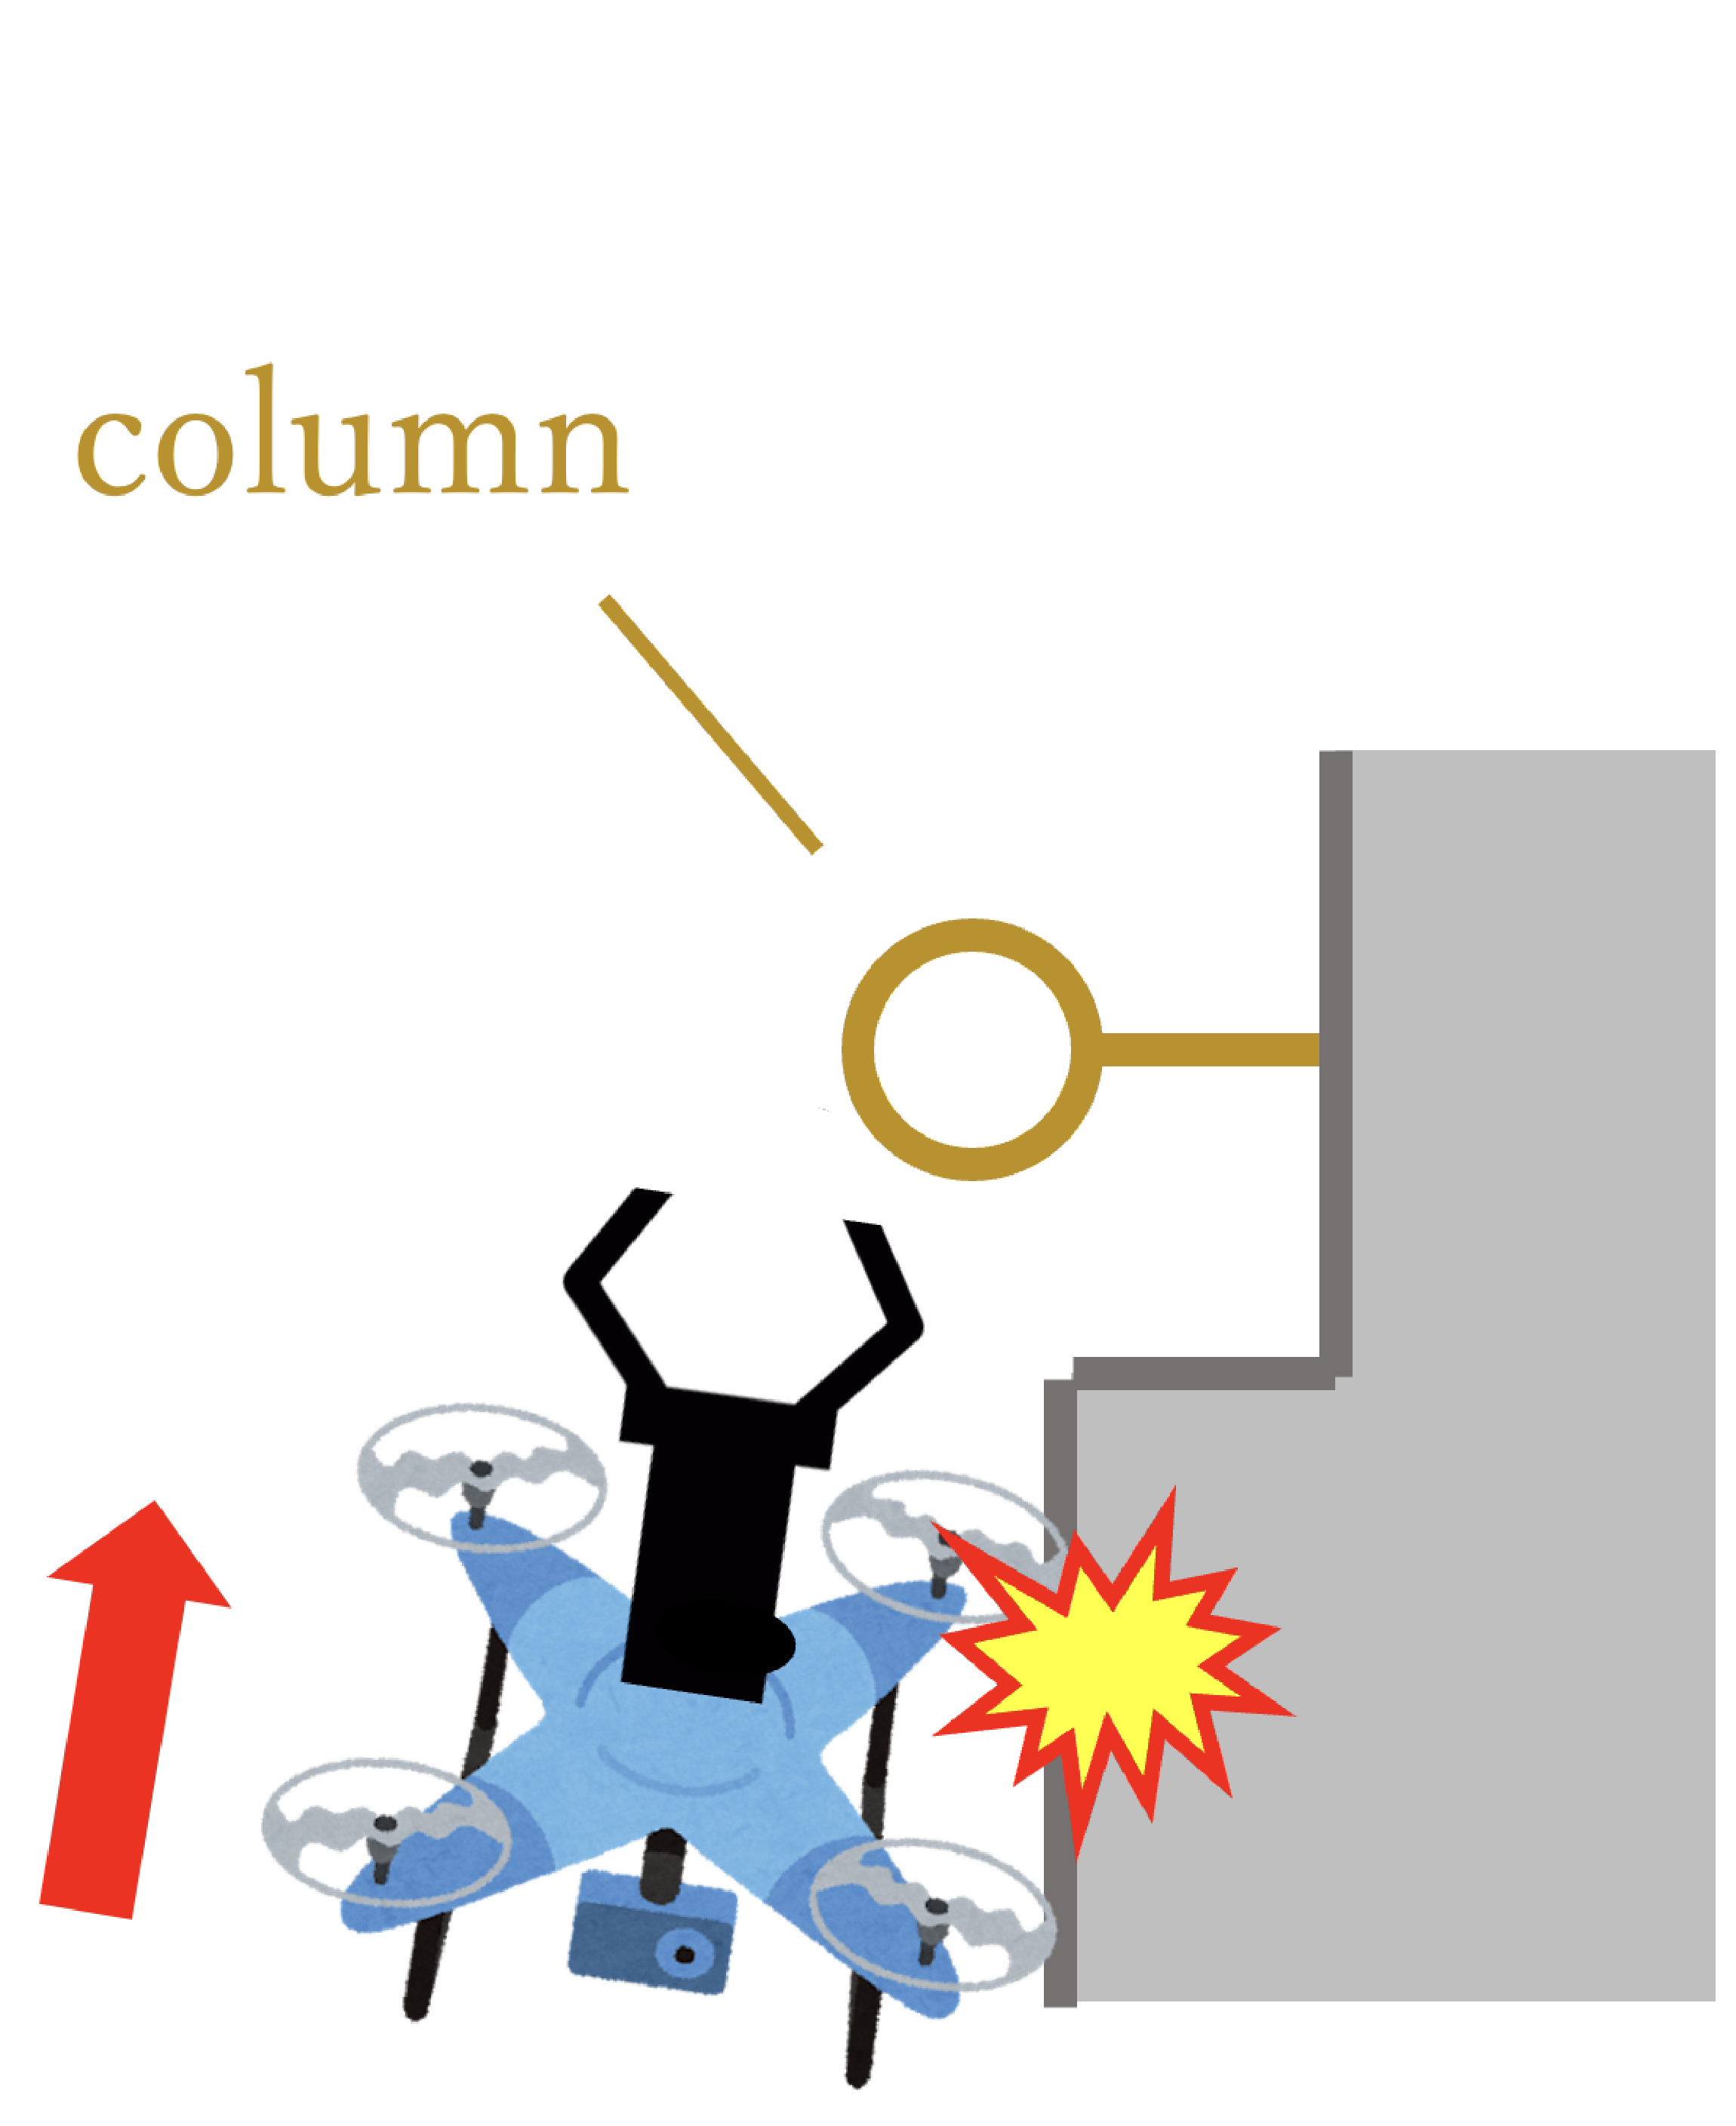
\includegraphics[width=\textwidth]{figs/collision.eps}
    \vspace{-6mm}
    \caption{}
    \label{fig:pgimage}
  \end{subfigure}
  \begin{subfigure}{0.68\columnwidth}
    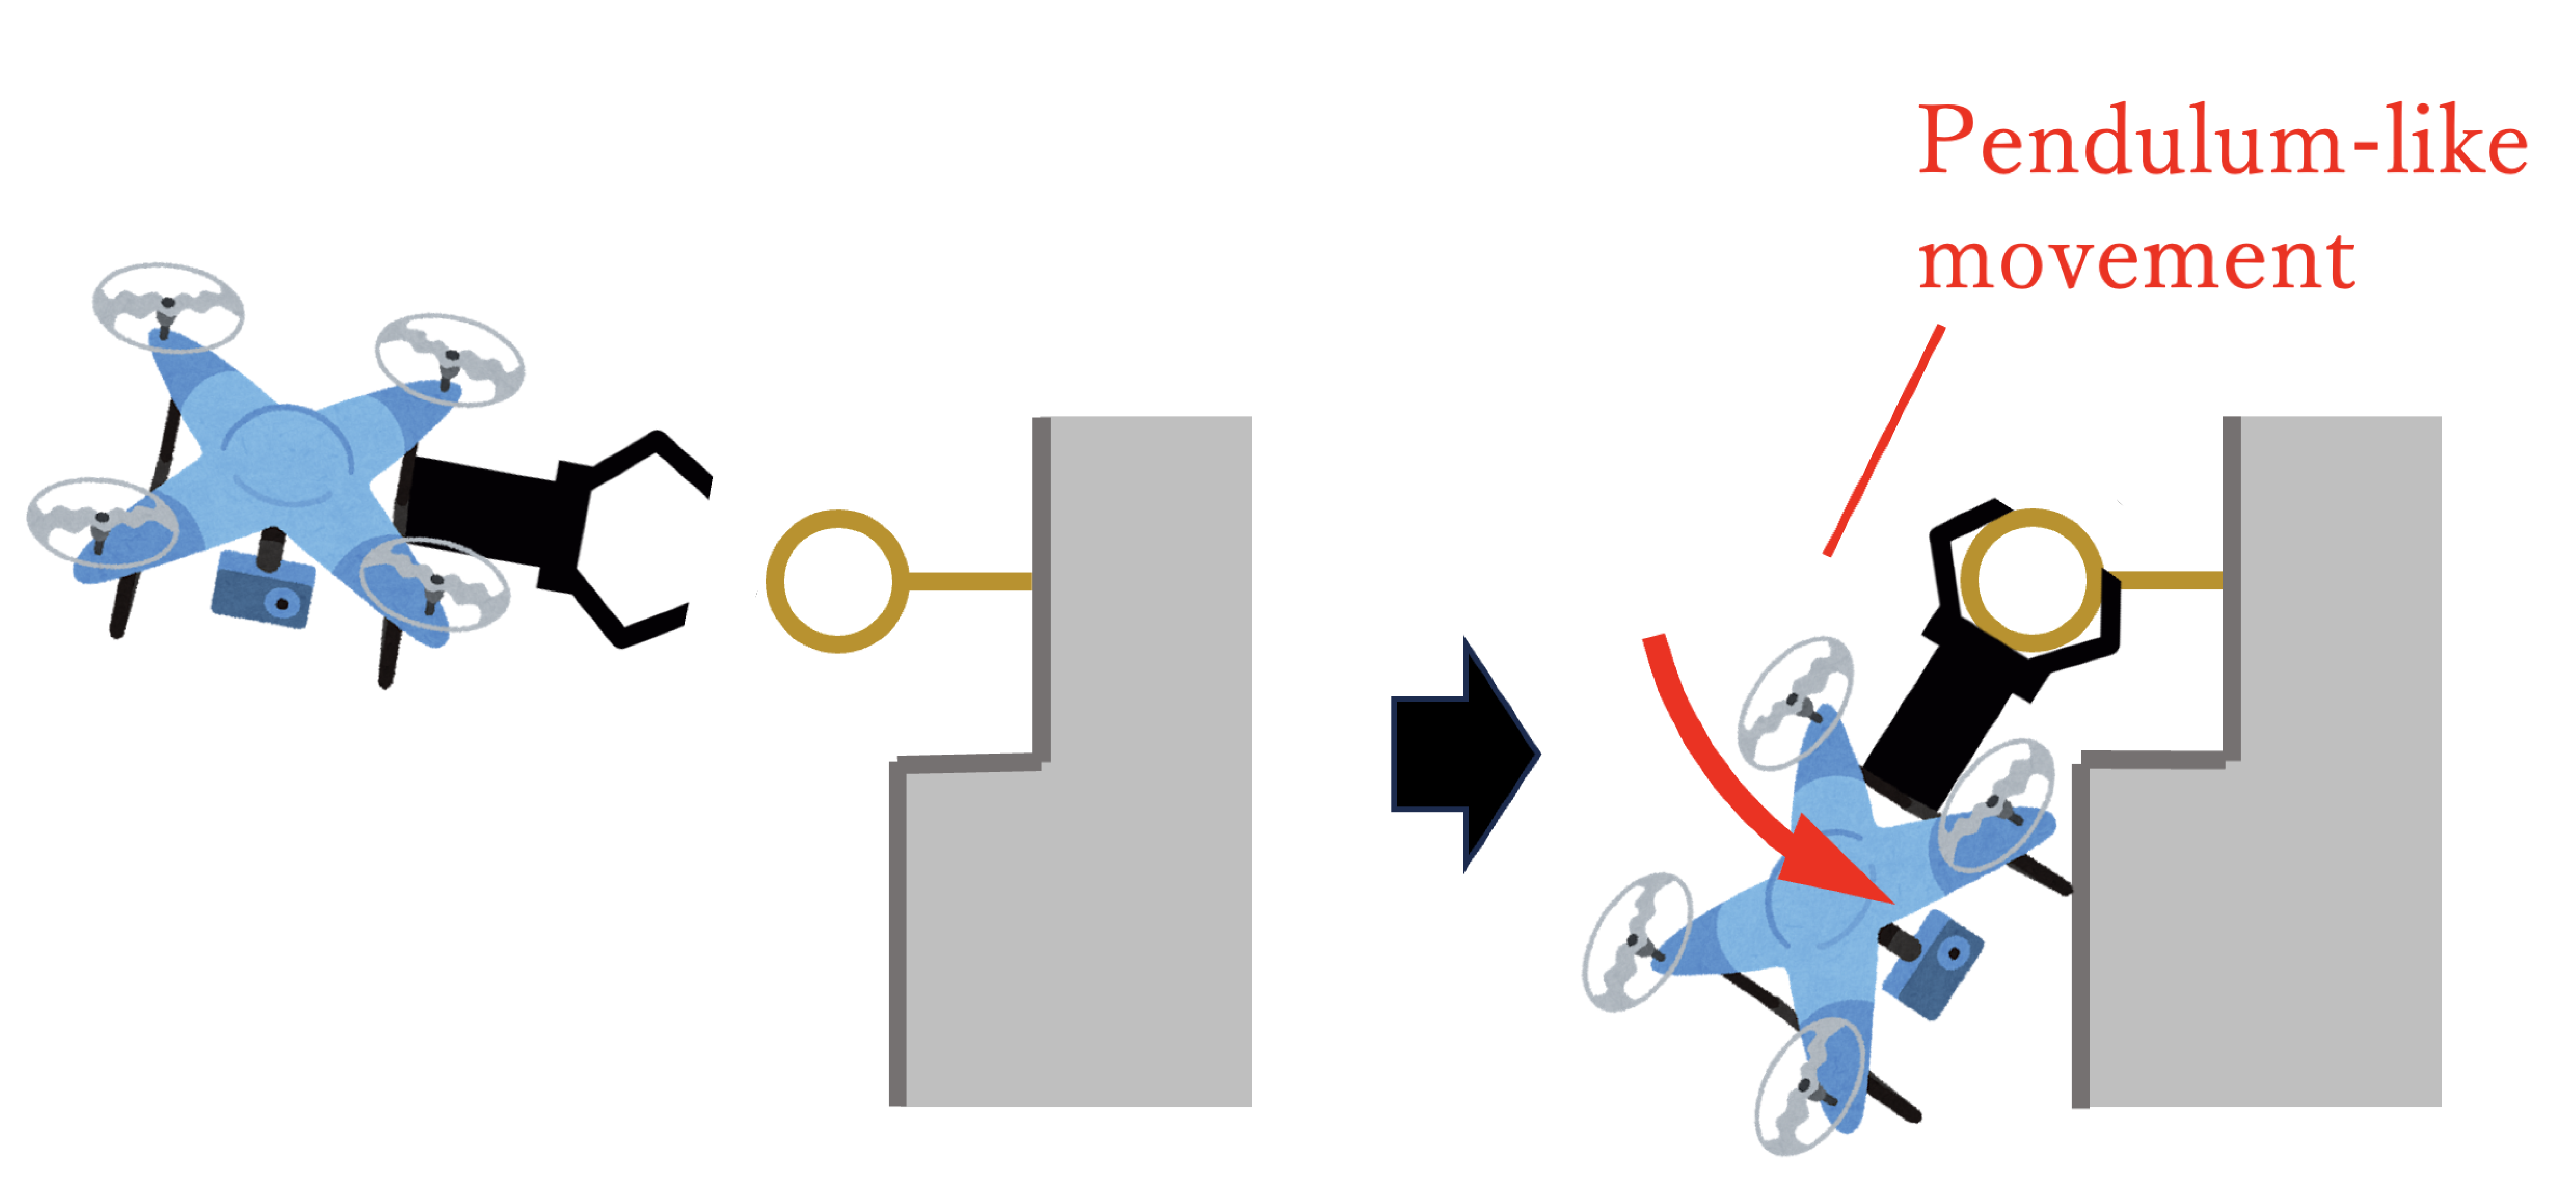
\includegraphics[width=\textwidth]{figs/perching_grasping.eps}
    \vspace{-6mm}
    \caption{}
    \label{fig:pgimage}
  \end{subfigure}
  \vspace{2mm}
  \caption{Perching and grasping image}
  \vspace{-5mm}
\end{figure}
加えて、ハンド機構の軽量化を行うことで機体重量が低下するため、さらに消費電力を削減可能である。パーチングのためのハンド機構の駆動方式は弾性、腱駆動、自重の利用などに分けられるが、自重駆動では結合方向が厳しく限られ、弾性駆動ではハンドが発揮する力や指関節の角度の制御が難しい。一方で腱駆動はこれらの欠点を持たず、さらに高い機械的コンプライアンスや動力位置自由度の高さなど飛行ロボットに適した特性を備えているが、アクチュエータ数が多くなりやすい。よって本研究では、腱駆動機構および少数アクチュエータを用いたハンド機構を全駆動飛行ロボットの機体に対して水平に配置し、アプローチから結合、離陸、解離までの機体制御手法をペンデュラム・パーチングとして提案する。

また単一機体による複数タスク実行に関して、既存研究では予め特定タスク専用のツールを組み込んだ機体を使用するものが多く、タスク数に応じてペイロードが圧迫される。この問題はアタッチメント交換方式により解決可能であり、事前に予測しえない形状のツールや物体の把持が可能な飛行ロボットの研究がGripper Droneとして進められている。先述したパーチングのための手先機構とGripperをともに飛行ロボットに搭載することで、消費電力の低減と複数タスクの実行を両立可能であると考えられる。しかしこれらのハンドの機能が独立している場合では、パーチング機構が飛行中に無駄なペイロードとなるなどの問題があり、最適な設計とは言えない。よって本研究では、パーチングと物体把持をともに行えるハンド機構を開発し、飛行ロボットに搭載する。

本研究のコントリビューションは以下のとおりである。

\begin{itemize}
  \item パーチングと従動的な物体把持が可能な飛行ロボットのための軽量な単一動力腱駆動ハンドの設計を提案する。
  \item 水平方向を中心とする多方向からのペンデュラム・パーチングおよび垂直状態からの離陸のための動作設計を提案する。
  \item 提案したハンドを搭載した飛行ロボットを用いてパーチングおよび離陸の実証実験を行った。
\end{itemize}

\section{ハンドの設計}
\subsection{ハンドの力学モデル}
\vspace{-4mm}
\begin{figure}[h]
  \centering
  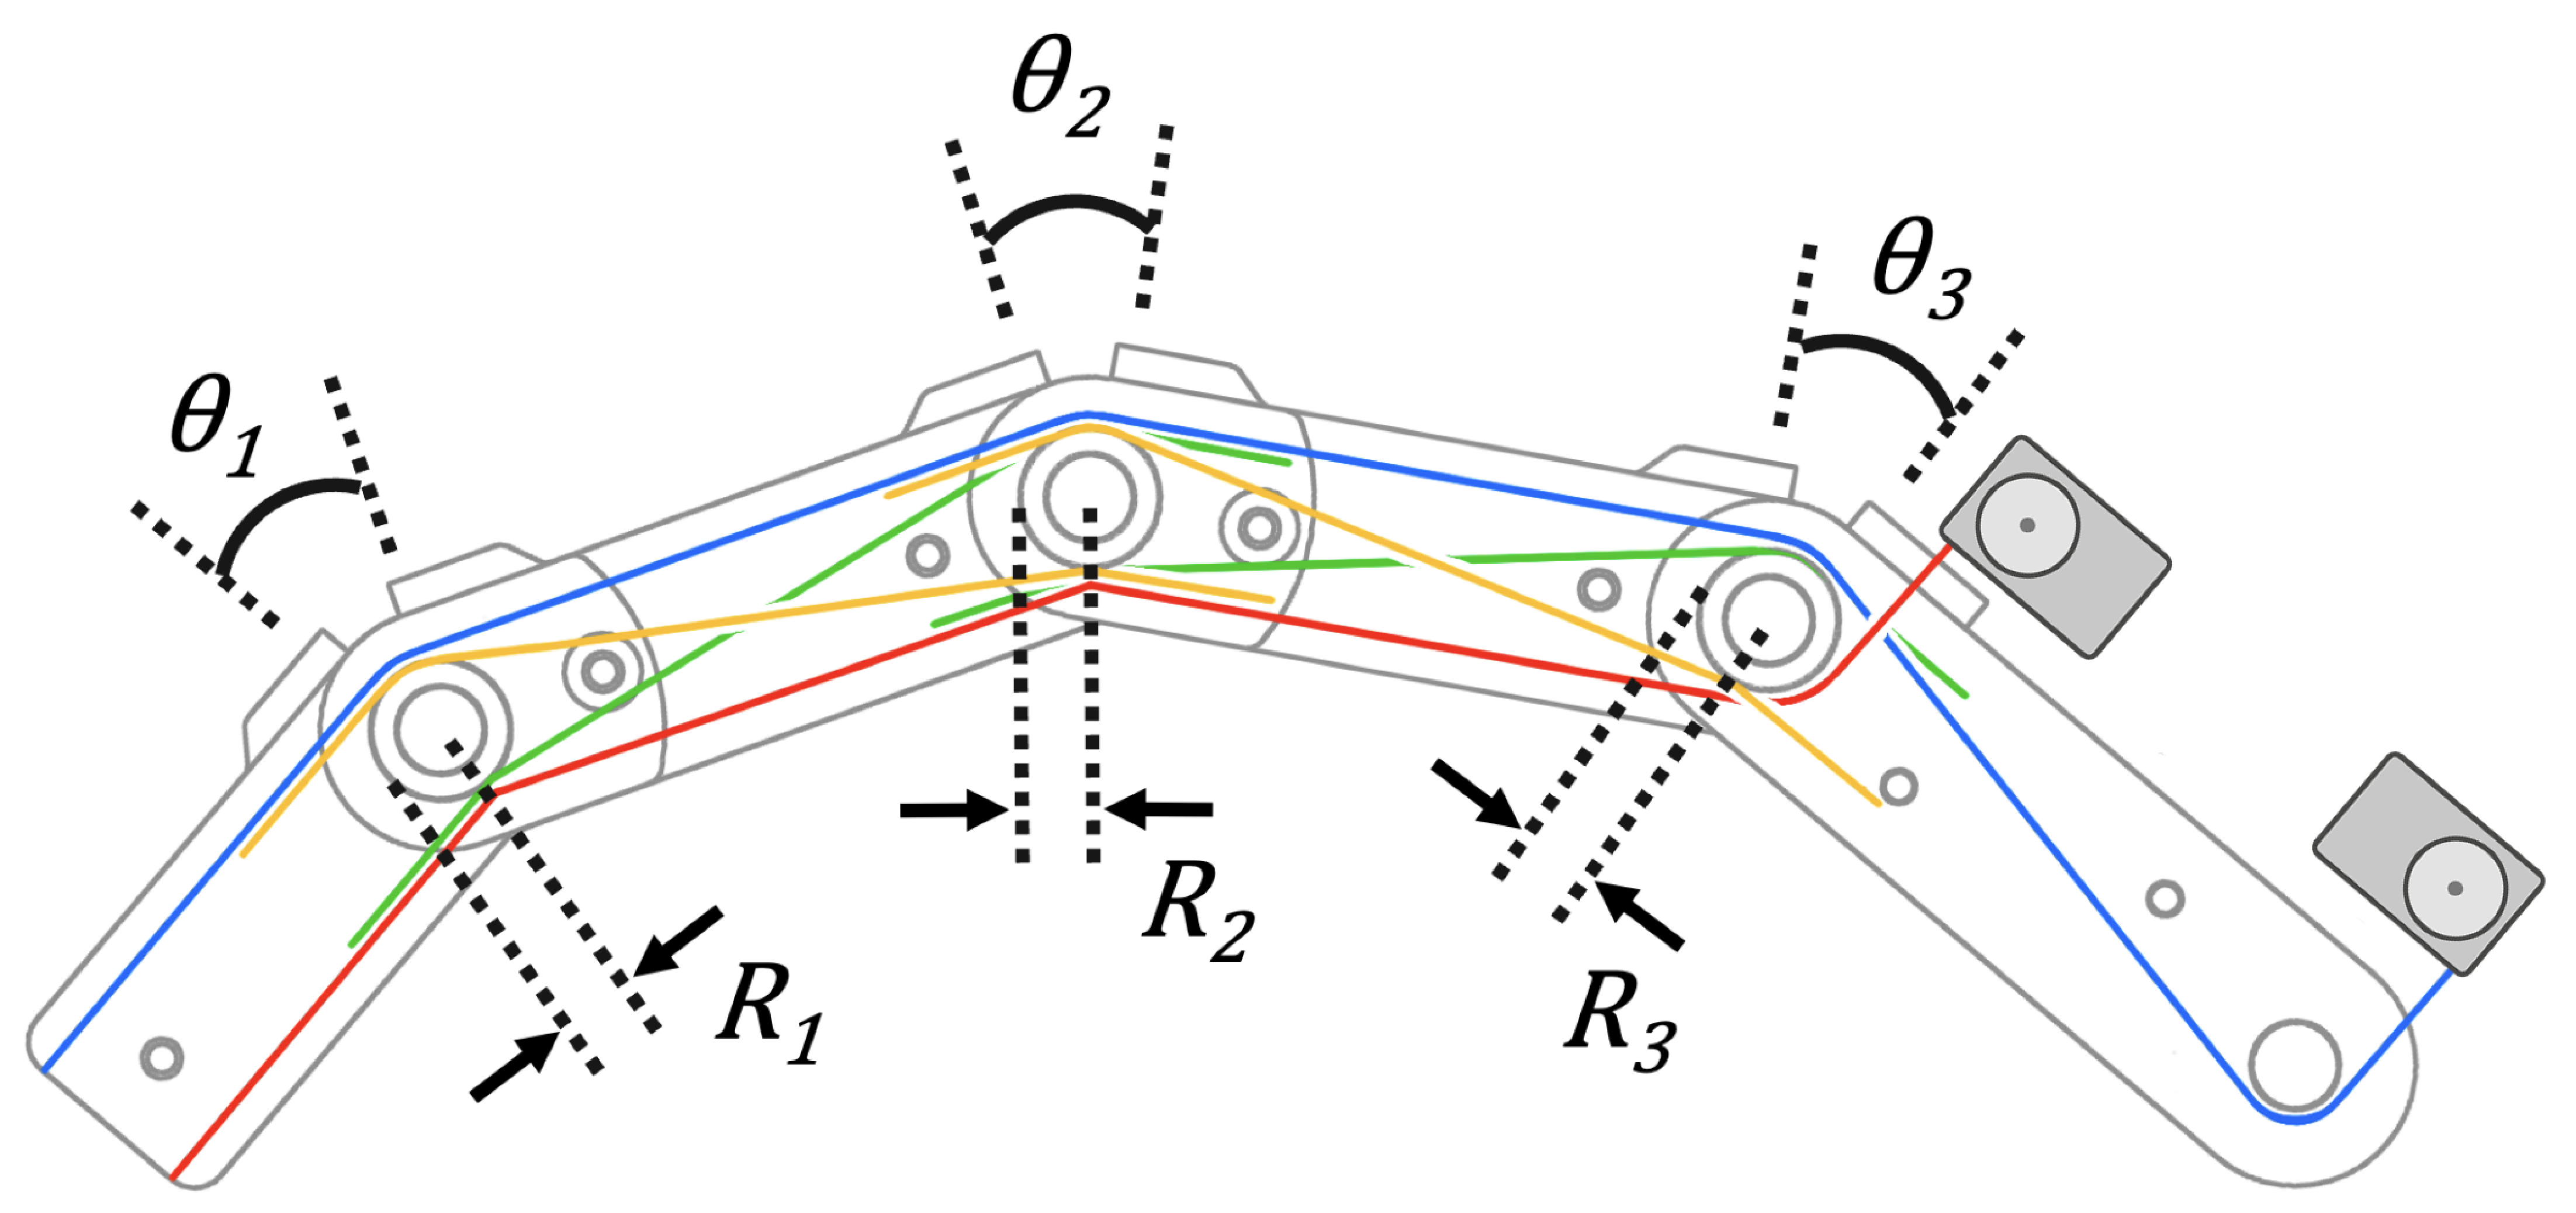
\includegraphics[width=0.8\columnwidth]{figs/cs-tdm.eps}
  \caption{CS-TDM finger module}
  \label{fig:cs-tdm}
  \vspace{-2mm}
\end{figure}
一般的な全駆動腱駆動では関節数と自由度は同一であり、関節数と同数以上のアクチュエータが必要となるため機構全体の重量が大きく、飛行ロボットには適さない。軽量かつ従動性を持ち少数のアクチュエータで駆動可能な腱駆動機構として、本研究では可制御半腱駆動(CS-TDM)を用いる。CS-TDMは劣駆動ながら物体把持に伴って形状が一意に定まるため、従動的に強い把持を行うことができ、力学モデルは腱の伸長$\bm{l}$、関節角度$\bm{\theta}$、アクチュエータ回転角度$\bm{\phi}$を用いて以下のように表される。
\vspace{-2mm}
\begin{equation}
  \left[ \begin{array}{c} \bm{l}_\text{a}\\ \bm{l}_\text{p} \end{array} \right] = \left[ \bm{J}_j \right] \bm{\dot{\theta}} + \left[ \bm{J}_s \right] \bm{\dot{\phi}} = \left[ \begin{array}{c} \bm{J}_\text{ja}\\ \bm{J}_\text{jp} \end{array} \right]  \bm{\dot{\theta}} + \left[ \begin{array}{c} \bm{J}_\text{sa}\\ \bm{0} \end{array} \right] \bm{\dot{\phi}}
  \vspace{-2mm}
  \label{equ:lmatrix}
\end{equation}
ただし、$\bm{J}_j、\bm{J}_s$はそれぞれ関節・アクチュエータプーリ径に依存する定数行列であり、添字$a$は駆動腱、$p$は受動腱に関する部分であることを表す。図\ref{fig:cs-tdm}に示したCS-TDMの構成条件は$rank\bm{J}_j = 3$かつ$0 < rank\bm{J}_\text{ja} < 3$であり、腱の伸長を0、関節プーリ径を$R_1 = R_2 = R_3$とし、式\ref{equ:lmatrix}の受動腱部分を抜き出して積分した形に変形すると、以下のように表される。
\vspace{-2mm}
\begin{equation}
  \bm{0} = \left[ \begin{array}{cccc} R_1 & 0 \\
    0 & R_1
  \end{array} \right]
  \left[ \begin{array}{c} \theta_1 - \theta_2 \\
    \theta_2 - \theta_3
  \end{array} \right]
  \label{passivematrixshort}
  \vspace{-2mm}
\end{equation}
ゆえに$\theta_1 = \theta_2 = \cdots = \theta_N$が導かれる。そこで本研究では人間の指構造と同一の4リンクからなるCS-TDMを構築し、関節プーリ径の統一により指形状を直線-正方折り畳み状態間で遷移可能とする。これにより、各指を2アクチュエータで駆動できる。

\subsection{トライフォース機構}
Neginらにより、レバー状の差動機構を用いて劣駆動ハンド機構を少数のアクチュエータで稼働する既存研究が提案されている。しかしこの機構では4本の指モジュールに対して差動機構の自由度が2であるため、物体把持時のハンド形状は指モジュールの初期状態に依存する。従って、物体形状によっては輪郭に従動的な追従を行えない。本研究ではこの課題を解決するため、より自由度の高い差動装置を利用することを考える。

図\ref{fig:differential}に示すように、三角形状の2次元差動板に球体関節を接続することで自由度4の差動機構を構築可能となるが、主腱まわりの回転が与える影響は小さいため実際の自由度は3とみなせる。故にこの差動機構により、前項のCS-TDMモジュールを用いて構築した3指ハンドの各指を初期状態によらない任意の状態へ従動的に駆動しうる。図\ref{fig:diff_2}のように差動板と屈腱の接点の座標をとると、差動機構の並進・回転により各指が任意の状態をとれる条件は屈腱の最大変位$d_\text{max}$を用いて以下のように表される。
\vspace{-2mm}
\begin{equation}
  0 < \frac{d_{\text{max}}}{r_{\text{1z}} - r_{\text{2z}}} < 1、0 < \frac{d_{\text{max}}}{2r_{\text{2y}}} < 1
  \label{equ:jouken}
  \vspace{-2mm}
\end{equation}
さらに伸腱に対しても差動機構を作成し、主腱により2枚の差動板とアクチュエータプーリを接続し両側駆動系とすることで、ハンド全体を単一のアクチュエータで駆動することが可能となる。これにより、最小動力数での駆動および従動的な物体把持が可能なハンドの設計条件が与えられた。本研究では、この差動機構をトライフォース機構と呼称する。

\begin{figure}[tb]
  \vspace{-2mm}
  \centering
  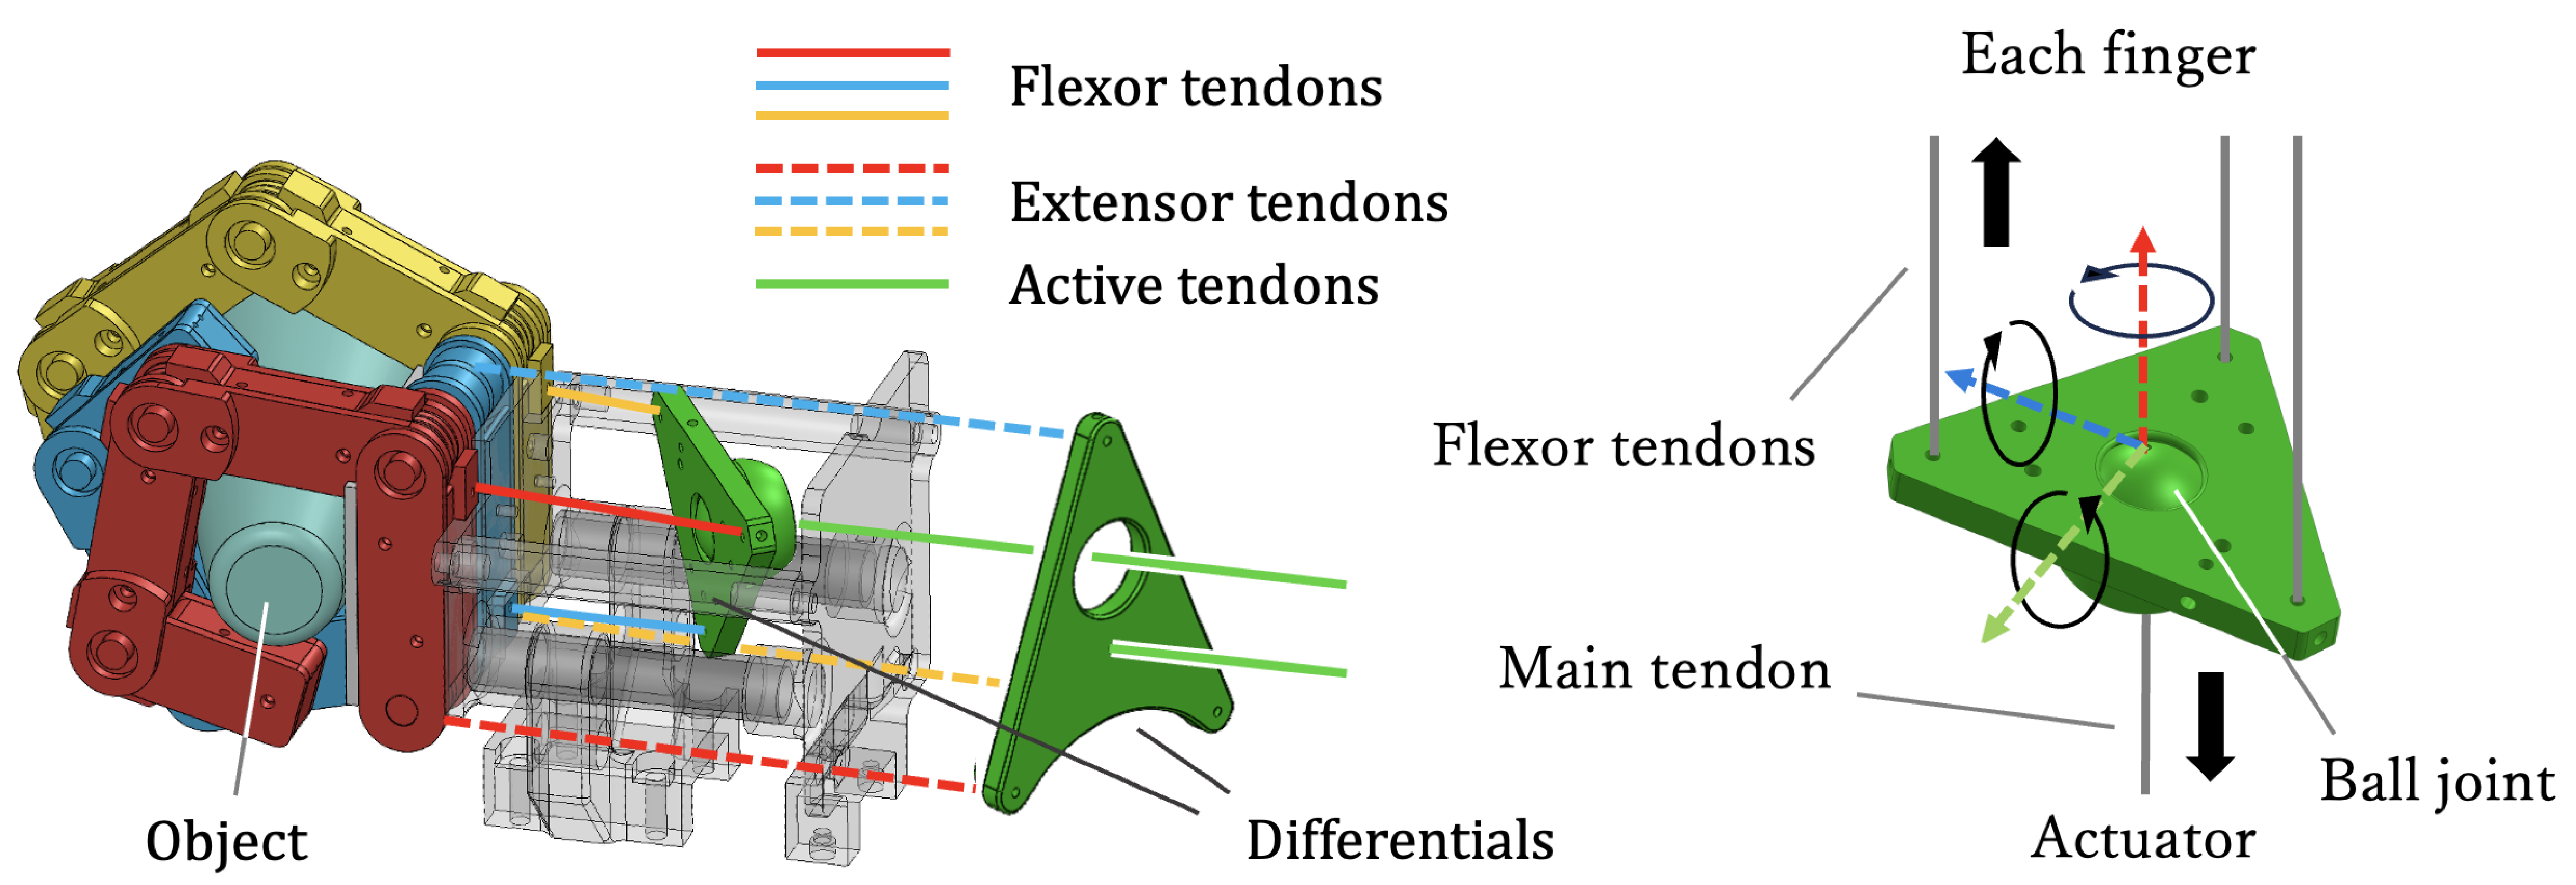
\includegraphics[width=0.8\columnwidth]{figs/differential.eps}
  \caption{CS-TDM finger module}
  \label{fig:differential}
\end{figure}
\begin{figure}[tb]
  \vspace{-2mm}
  \centering
  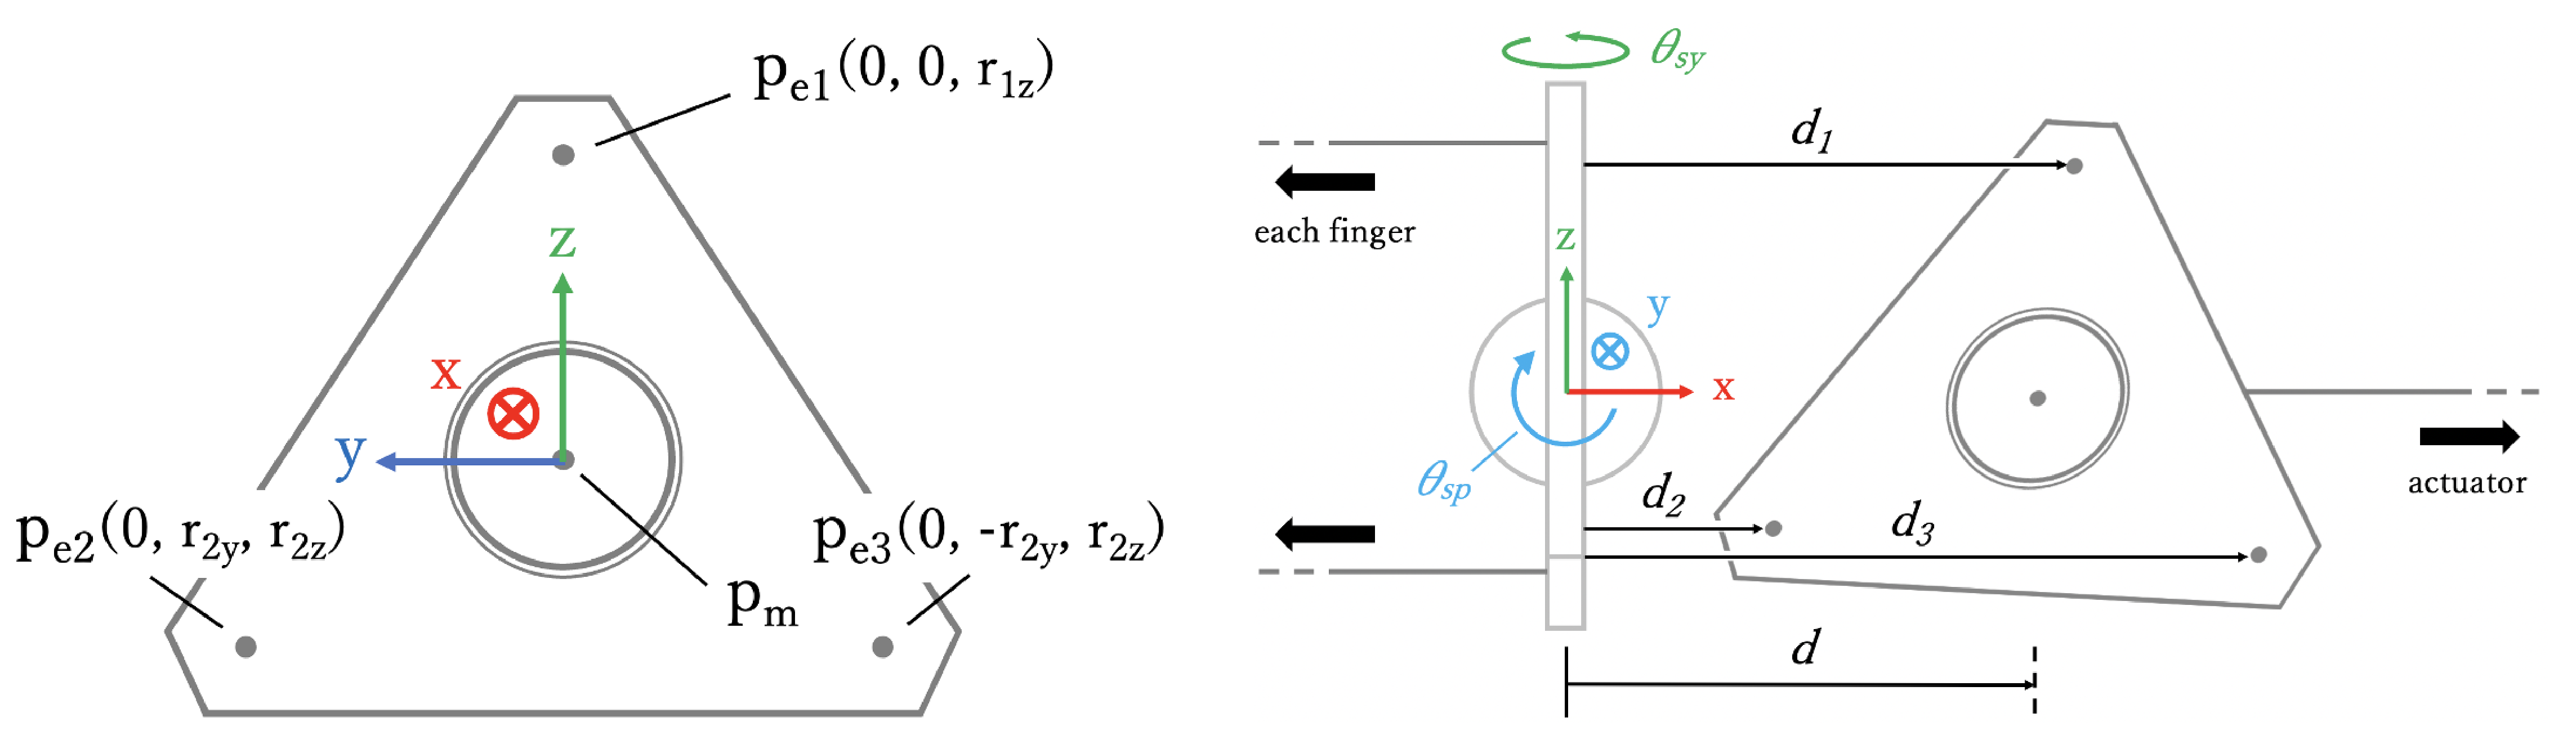
\includegraphics[width=0.8\columnwidth]{figs/diff_2.eps}
  \caption{two-dimensional differential}
  \label{fig:diff_2}
  \vspace{-2mm}
\end{figure}
\subsection{ハンドの支持可能重量}
\vspace{-2mm}
\begin{figure}[h]
  \centering
  \begin{subfigure}{0.3\columnwidth}
    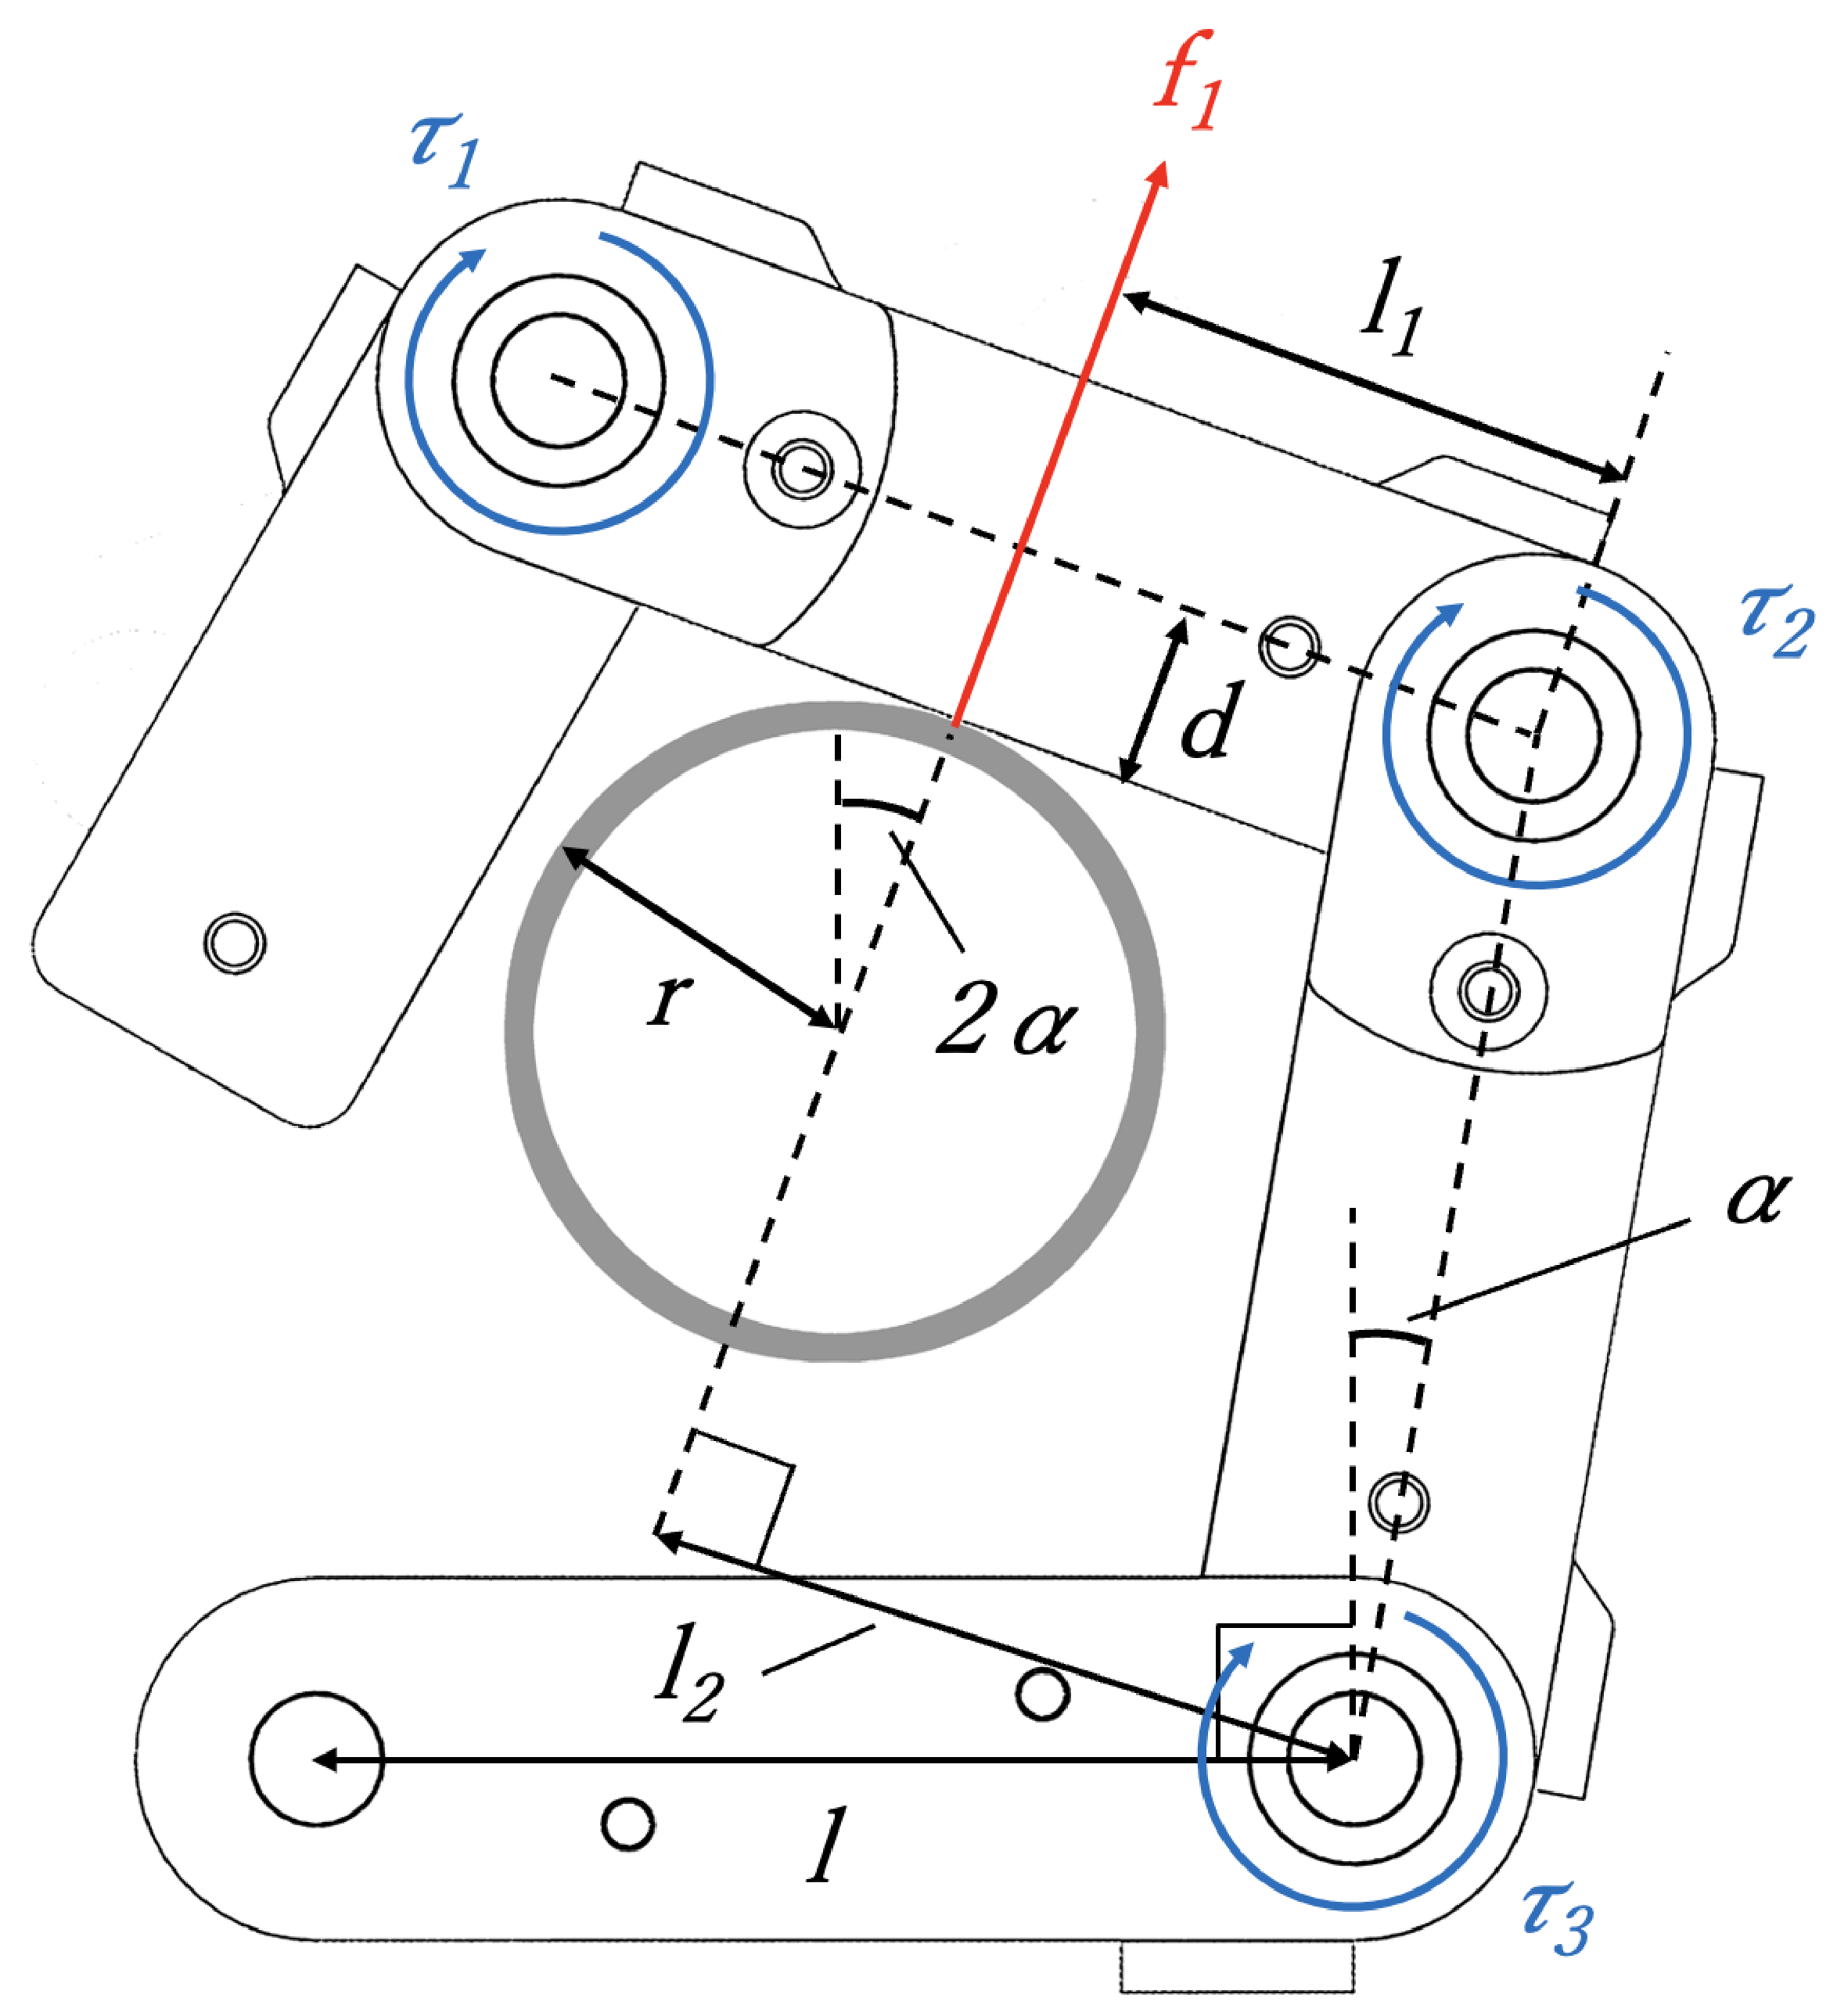
\includegraphics[width=\textwidth]{figs/weight1.eps}
    \caption{}
    \label{fig:weight1}
  \end{subfigure}
  \begin{subfigure}{0.6\columnwidth}
    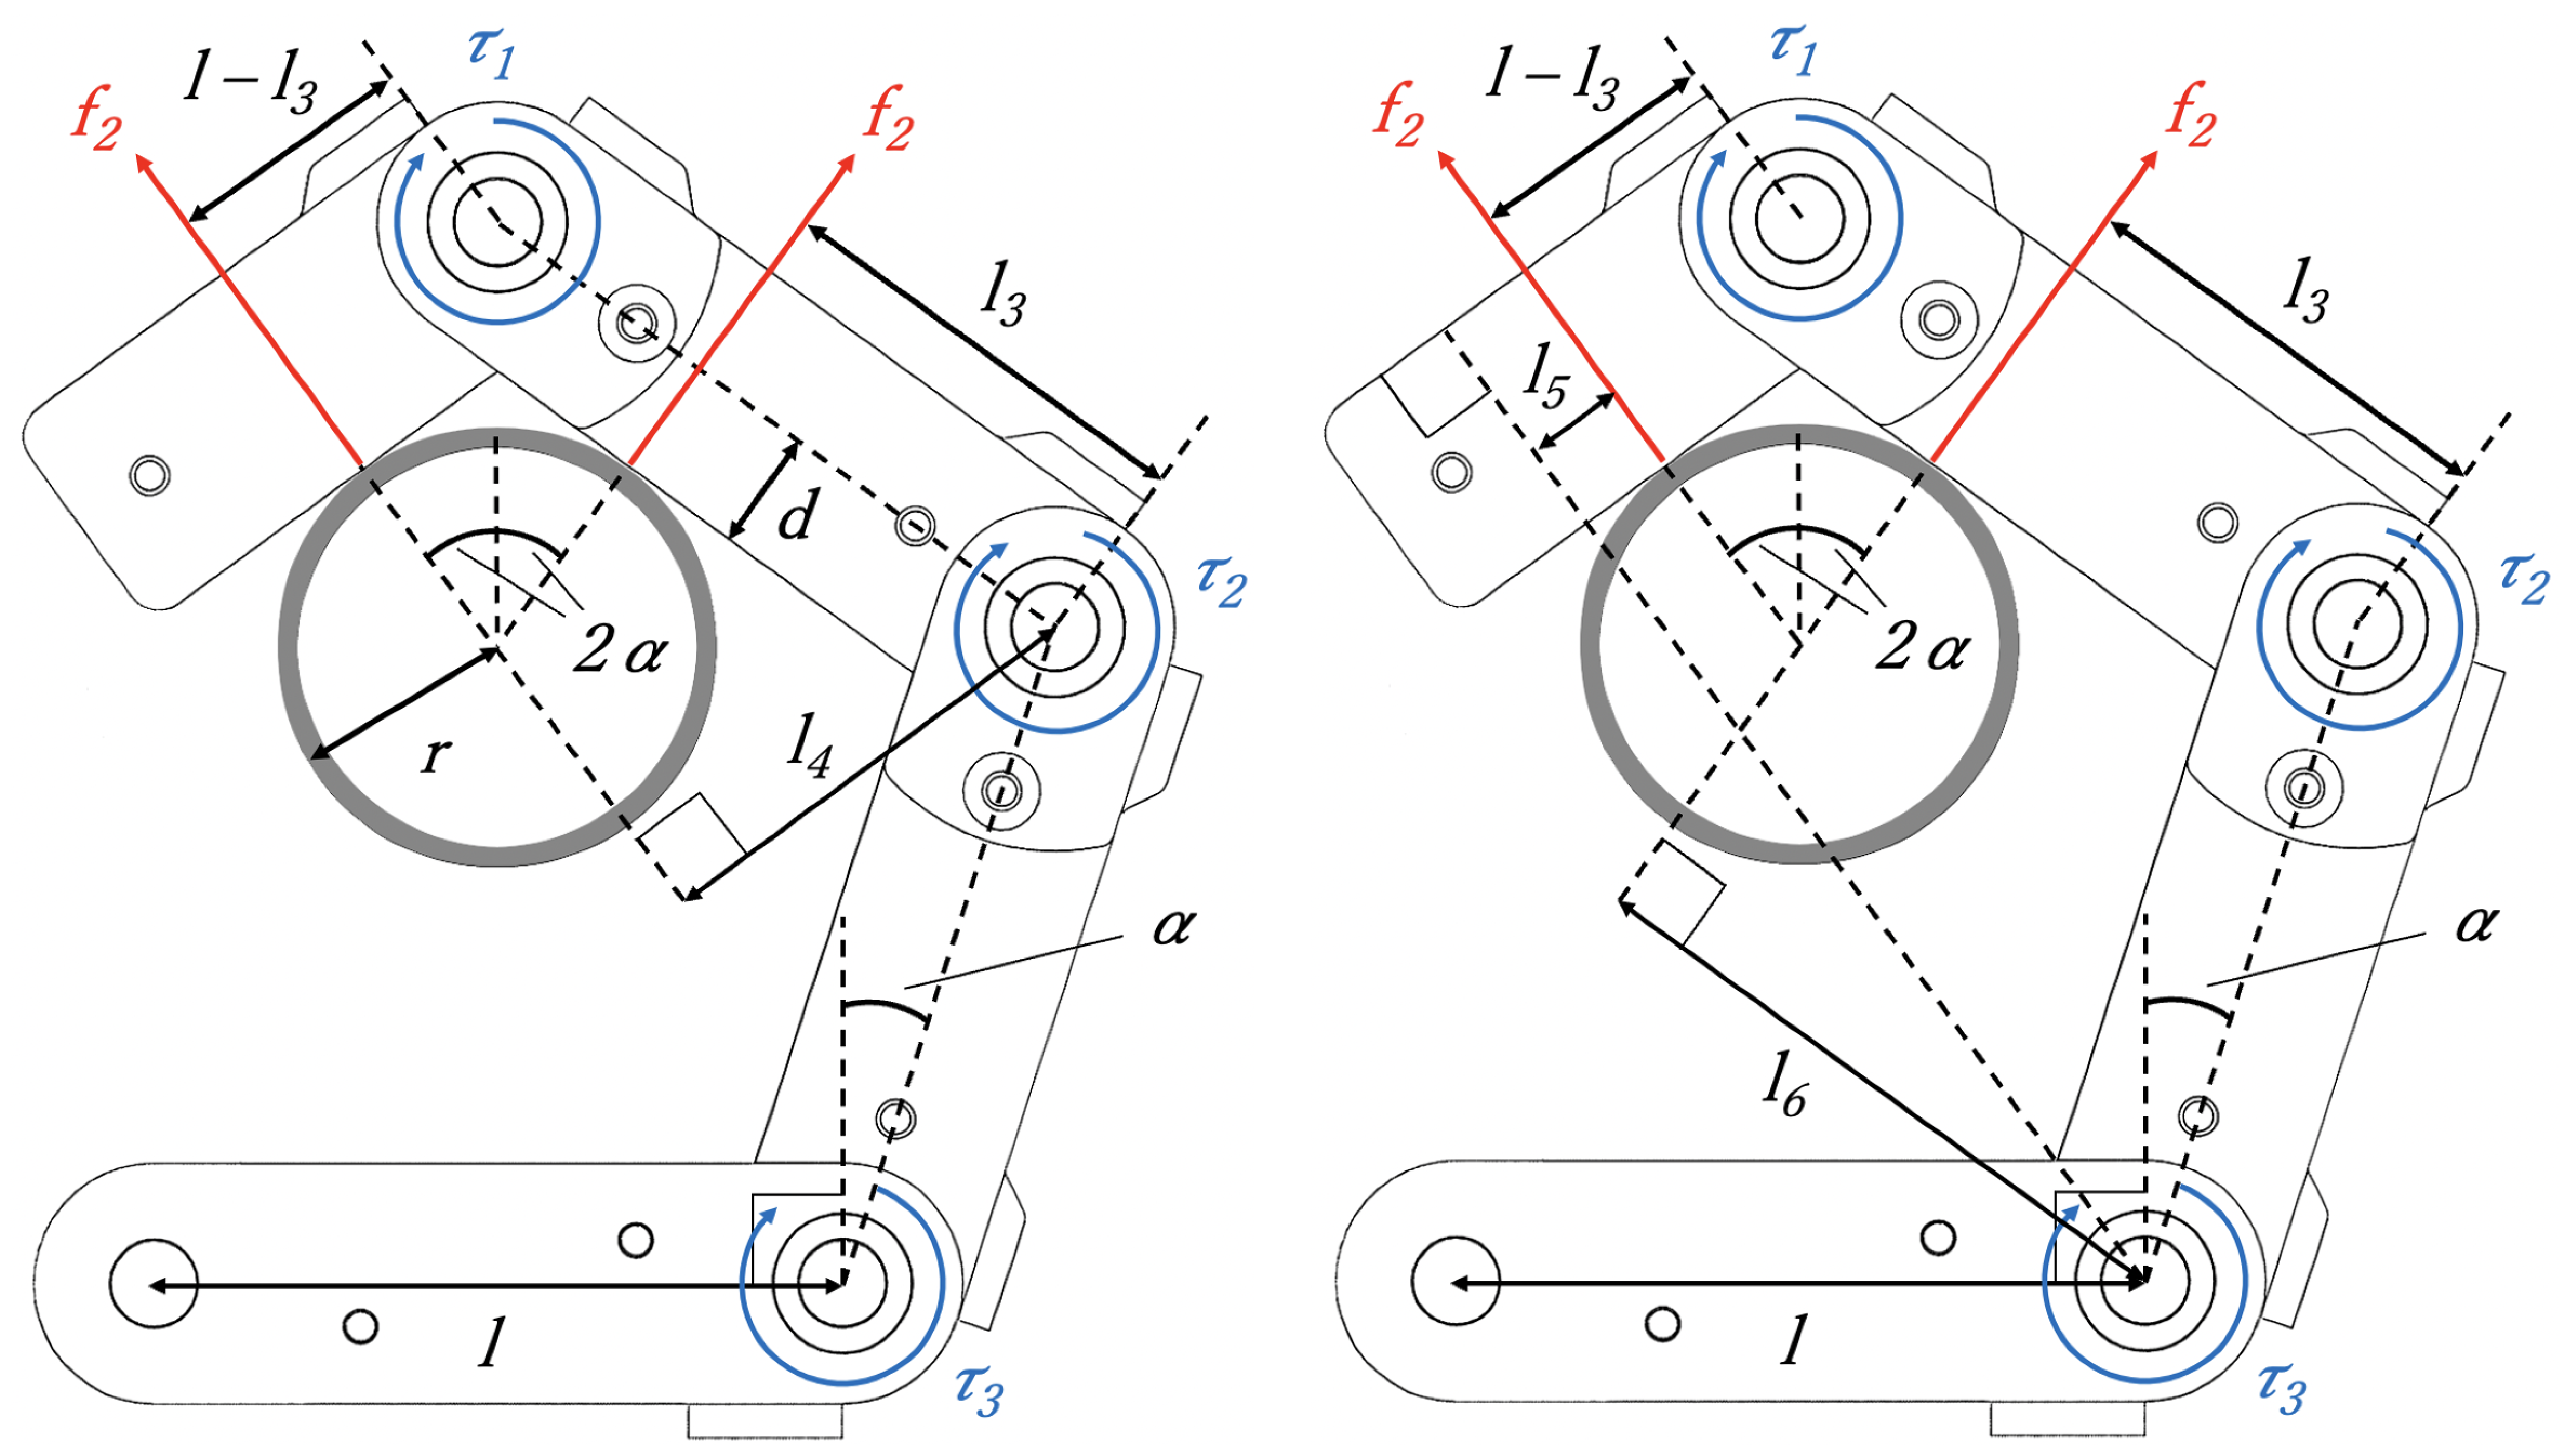
\includegraphics[width=\textwidth]{figs/weight2.eps}
    \caption{}
    \label{fig:weight2}
  \end{subfigure}
  \vspace{2mm}
  \caption{Hand load capacity}
  \vspace{-2mm}
\end{figure}
図\ref{fig:weight1}に示すような細い円柱形状の把持では、モーメントアーム$l_1、l_2$および指に働く力$f_1$は以下のように表される。
\vspace{-2mm}
\begin{equation}
  l_1 = \frac{l}{2\cos(2\alpha)}、l_2 = l_1 + l\sin(\alpha)、f_1 = \frac{mg}{3\cos(2\alpha)}
  \vspace{-2mm}
  \label{equ:euler}
\end{equation}
$\alpha$は指関節開き角、mは荷重であり、$l_1$は$\alpha$が十分に小さいとして近似した。ここでオイラーのベルト理論から、腱を関節プーリに巻きつけることにより張力が以下の式に従って上昇する。
\vspace{-2mm}
\begin{equation}
  T_\text{out} = T_\text{in} \, e^{\mu\delta}
  \vspace{-2mm}
\end{equation}
$\mu、\delta$は摩擦係数、巻き付け角度である。よって、重量支持の条件式はアクチュエータストールトルク$\tau_\text{st}$、減速比$c$、アクチュエータプーリ径$R_\text{gp}$および摩擦係数$\mu$を用いて書き表される。
\vspace{-2mm}
\begin{equation}
  3\frac{f_1l_1 + f_1l_2}{R_1} \leq c \frac{\tau_\text{st}}{R_\text{gp}} e^{\mu(2\pi + \alpha)}
  \vspace{-2mm}
  \label{equ:jouken}
\end{equation}
\begin{equation}
  m_{\text{maxa}} = \frac{\tau_{\text{st}} R_1 c e^{\mu(2\pi + \alpha)}}{g l R_{\text{gp}}} \cdot \frac{\cos^2(2\alpha)}{\sin(\alpha) \cos(2\alpha) + 1}
  \label{equ:mmaxa}
\end{equation}
$m_\text{maxa}$は$\alpha$の増加に伴って単調に減少するが、$\alpha = \pi/10$においてハンドは図\ref{fig:weight2}の状態に遷移し、最大荷重は以下のようである。
\vspace{-2mm}
\begin{equation}
  m_{\text{maxb}} = \frac{\tau_{\text{st}} R_1 c e^{\mu \frac{21\pi}{10}}}{g l R_{\text{gp}}} \cdot \frac{4 \cos^2(2\alpha)}{4\sin(\alpha)\cos(2\alpha) + 5\cos(2\alpha) - 1}
  \label{equ:mmaxb}
\end{equation}
ここで、$\alpha = \pi / 10$においては$m_\text{maxa} < m_\text{maxb}$であるため、支持可能重量のジャンプが起こると考えられる。よって、実際の設計においては$m_{maxb}$がパーチング過程においてハンドに作用する力を十分に上回る必要がある。
\section{飛行動作設計}
提案したペンデュラム・パーチングにおいて、機体はハンドを介して環境物体に拘束され、さらに垂直近傍まで大きく傾斜することがありうる。本項ではこのような特異状態下における機体の動作計画について述べる。

本研究で使用したベース機体は推力偏向機構を持つ8自由度の全駆動クアッドロータであり、目標機体位置に関するPID制御によるコントロールを行う。しかし機体が環境物体と結合した状態においては、目標位置入力への到達が必ずしも可能であるとは限らない。よって機体の目標pitch角度$\theta_p^\text{des}$を入力として取り、制御開始地点$\bm{r}^\text{bottom}$における機体のpitch、yaw角度$\theta_p、\theta_y$から機体が到達すべき目標位置$\bm{r}^\text{des}$を以下のように算出する。
\vspace{-2mm}
\begin{equation}
  \bm{r}^\text{des} = \bm{r}^\text{bottom} -
  \left[ \begin{array}{c} l_h(\cos(\theta_p^\text{des}) - \cos(\theta_p))\cos(\theta_y) \\
      l_h(\cos(\theta_p^\text{des}) - \cos(\theta_p))\sin(\theta_y) \\
      -l_h(\sin(\theta_p^\text{des}) - \sin(\theta_p))
    \end{array} \right]
  \vspace{-2mm}
  \label{eq:rset}
\end{equation}
\begin{figure}[tb]
  \centering
  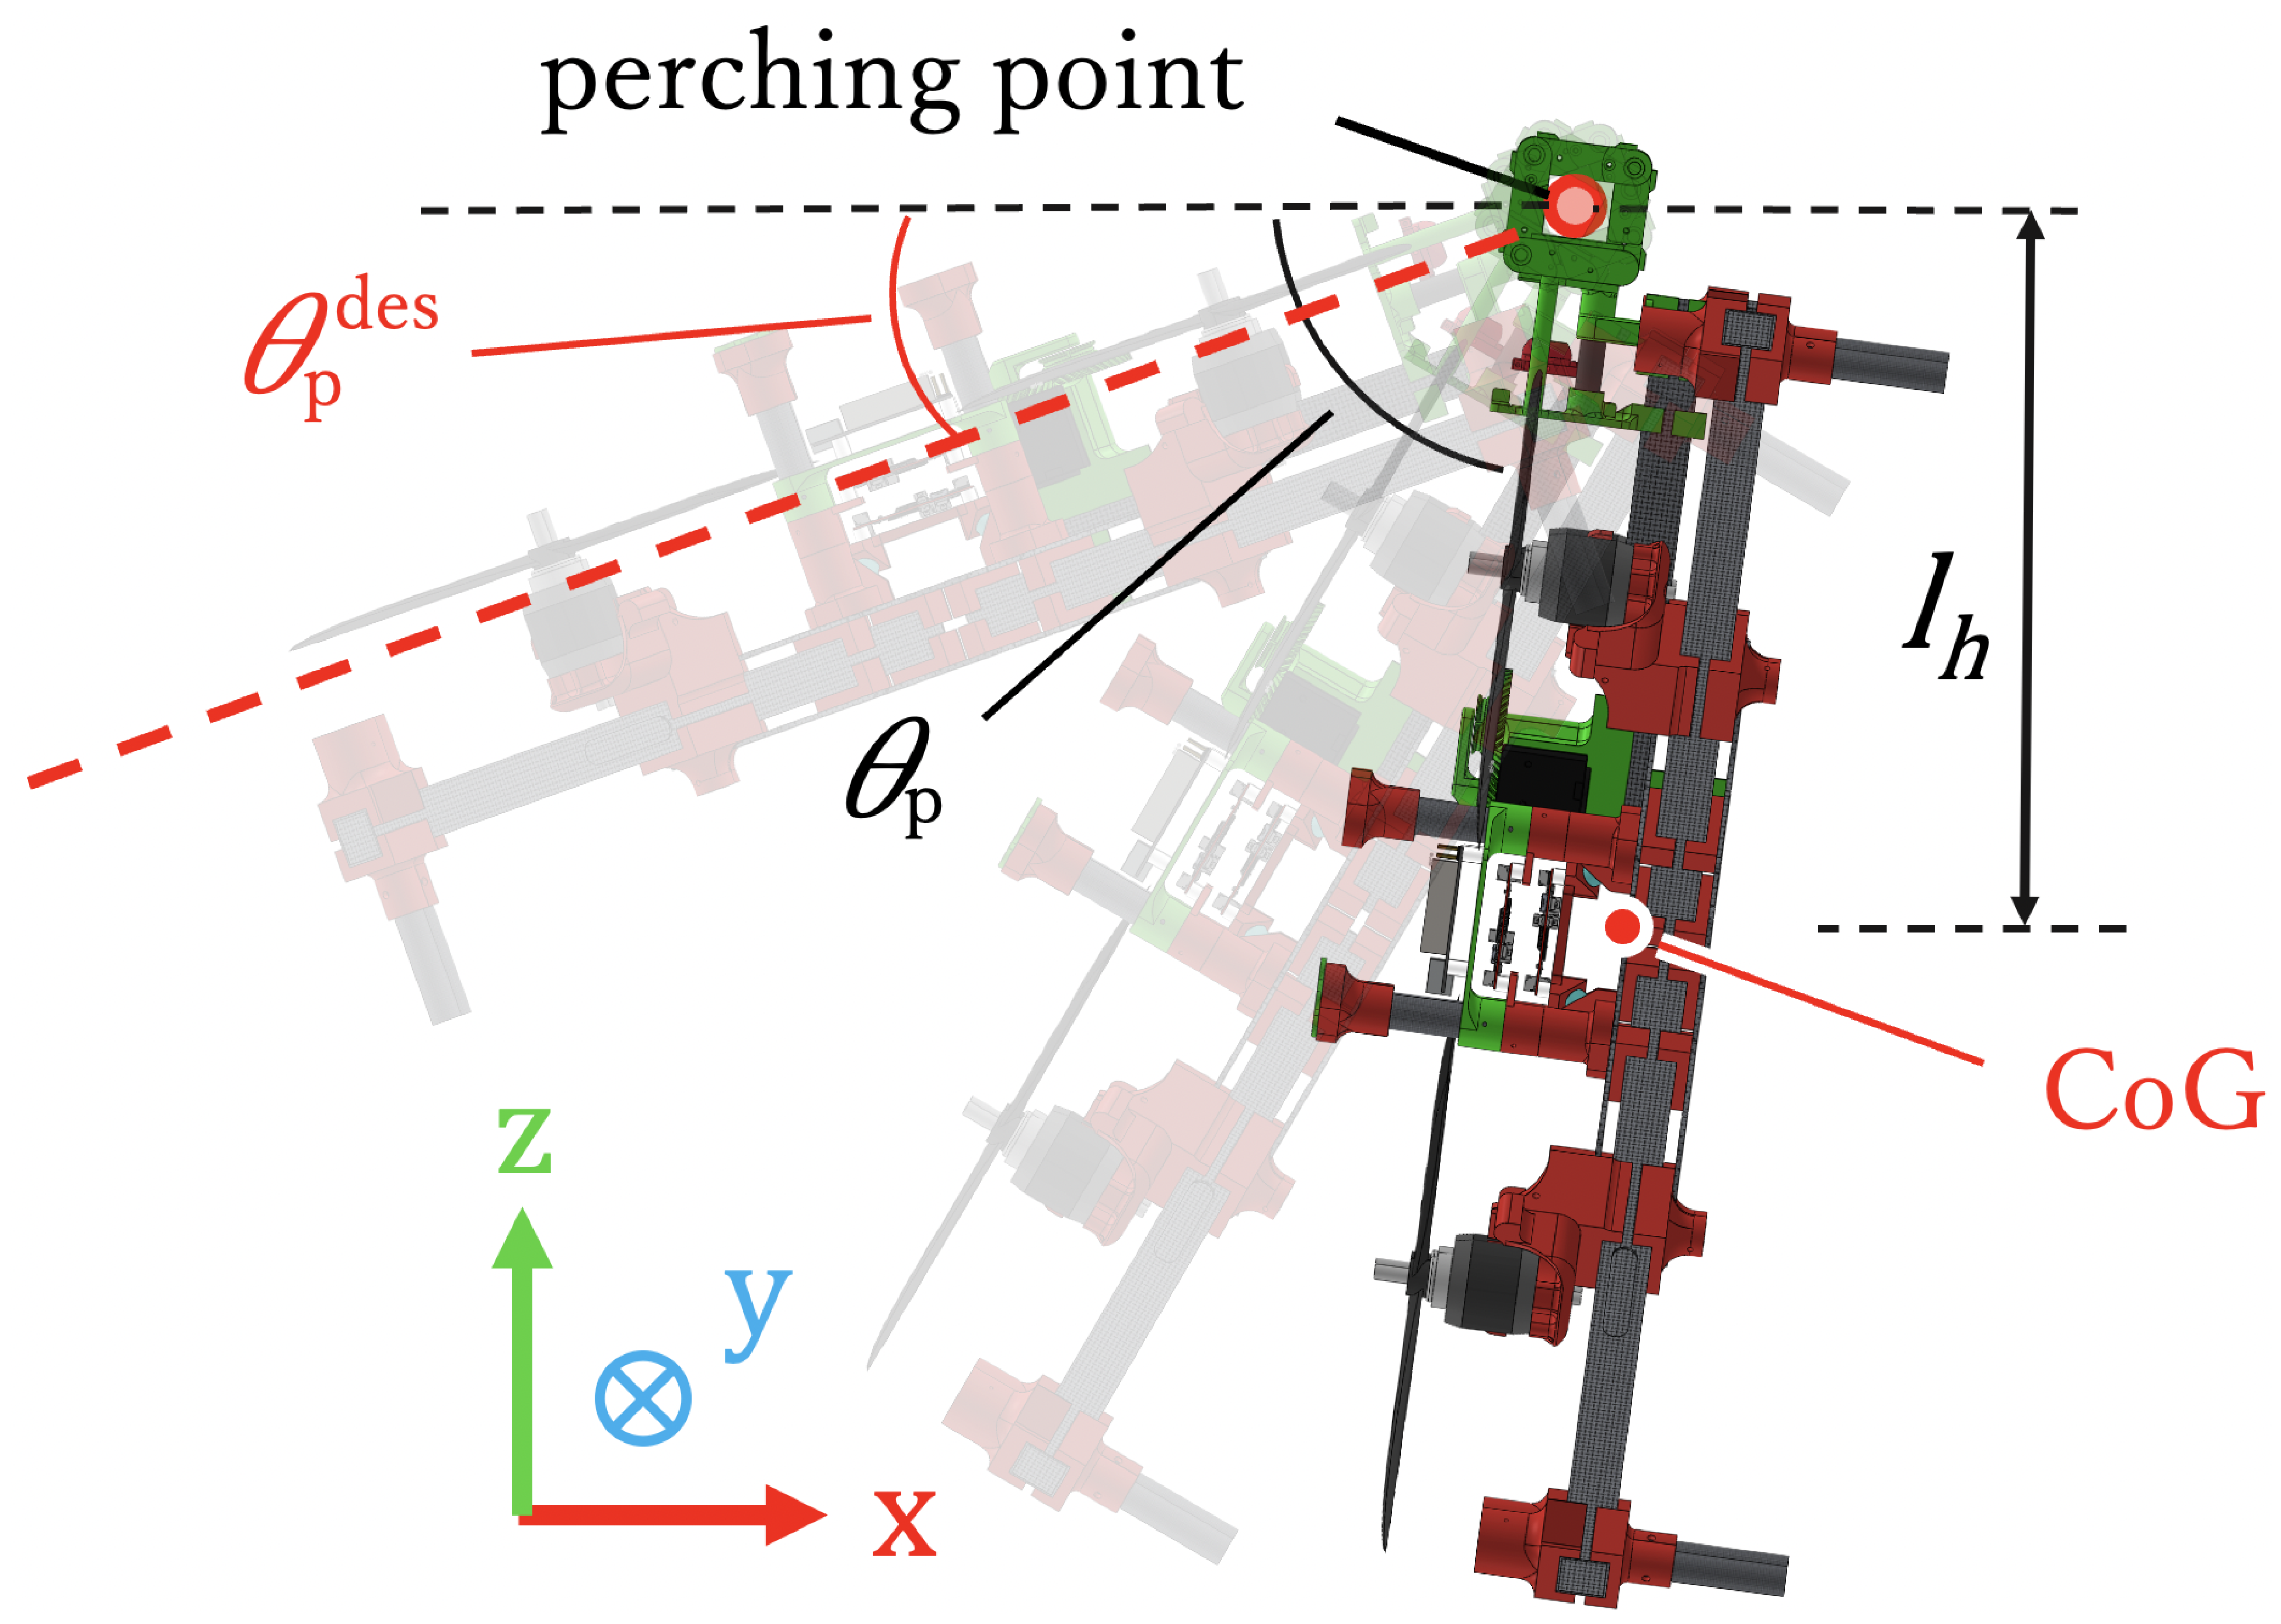
\includegraphics[width=0.6\columnwidth]{figs/rset.eps}
  \caption{Takeoff control in pendulum-perching}
  \vspace{-4mm}
  \label{fig:rset}
\end{figure}
これにより機体は推力の範囲内で任意のpitch角度に到達可能となるが、$\theta_p$と$\theta_p^\text{des}$が大きく異なる場合は離陸に時間を要するため、蓄積した積分要素により解離直後に飛行が不安定となりうる。よって結合中はz座標のみPID制御を行い、その他の制御要素についてはPD制御を行うことで離陸動作を安定化する。

\section{実験}
\subsection{ハンドの実制作と実装}
\vspace{-2mm}
\begin{figure}[h]
  \centering
  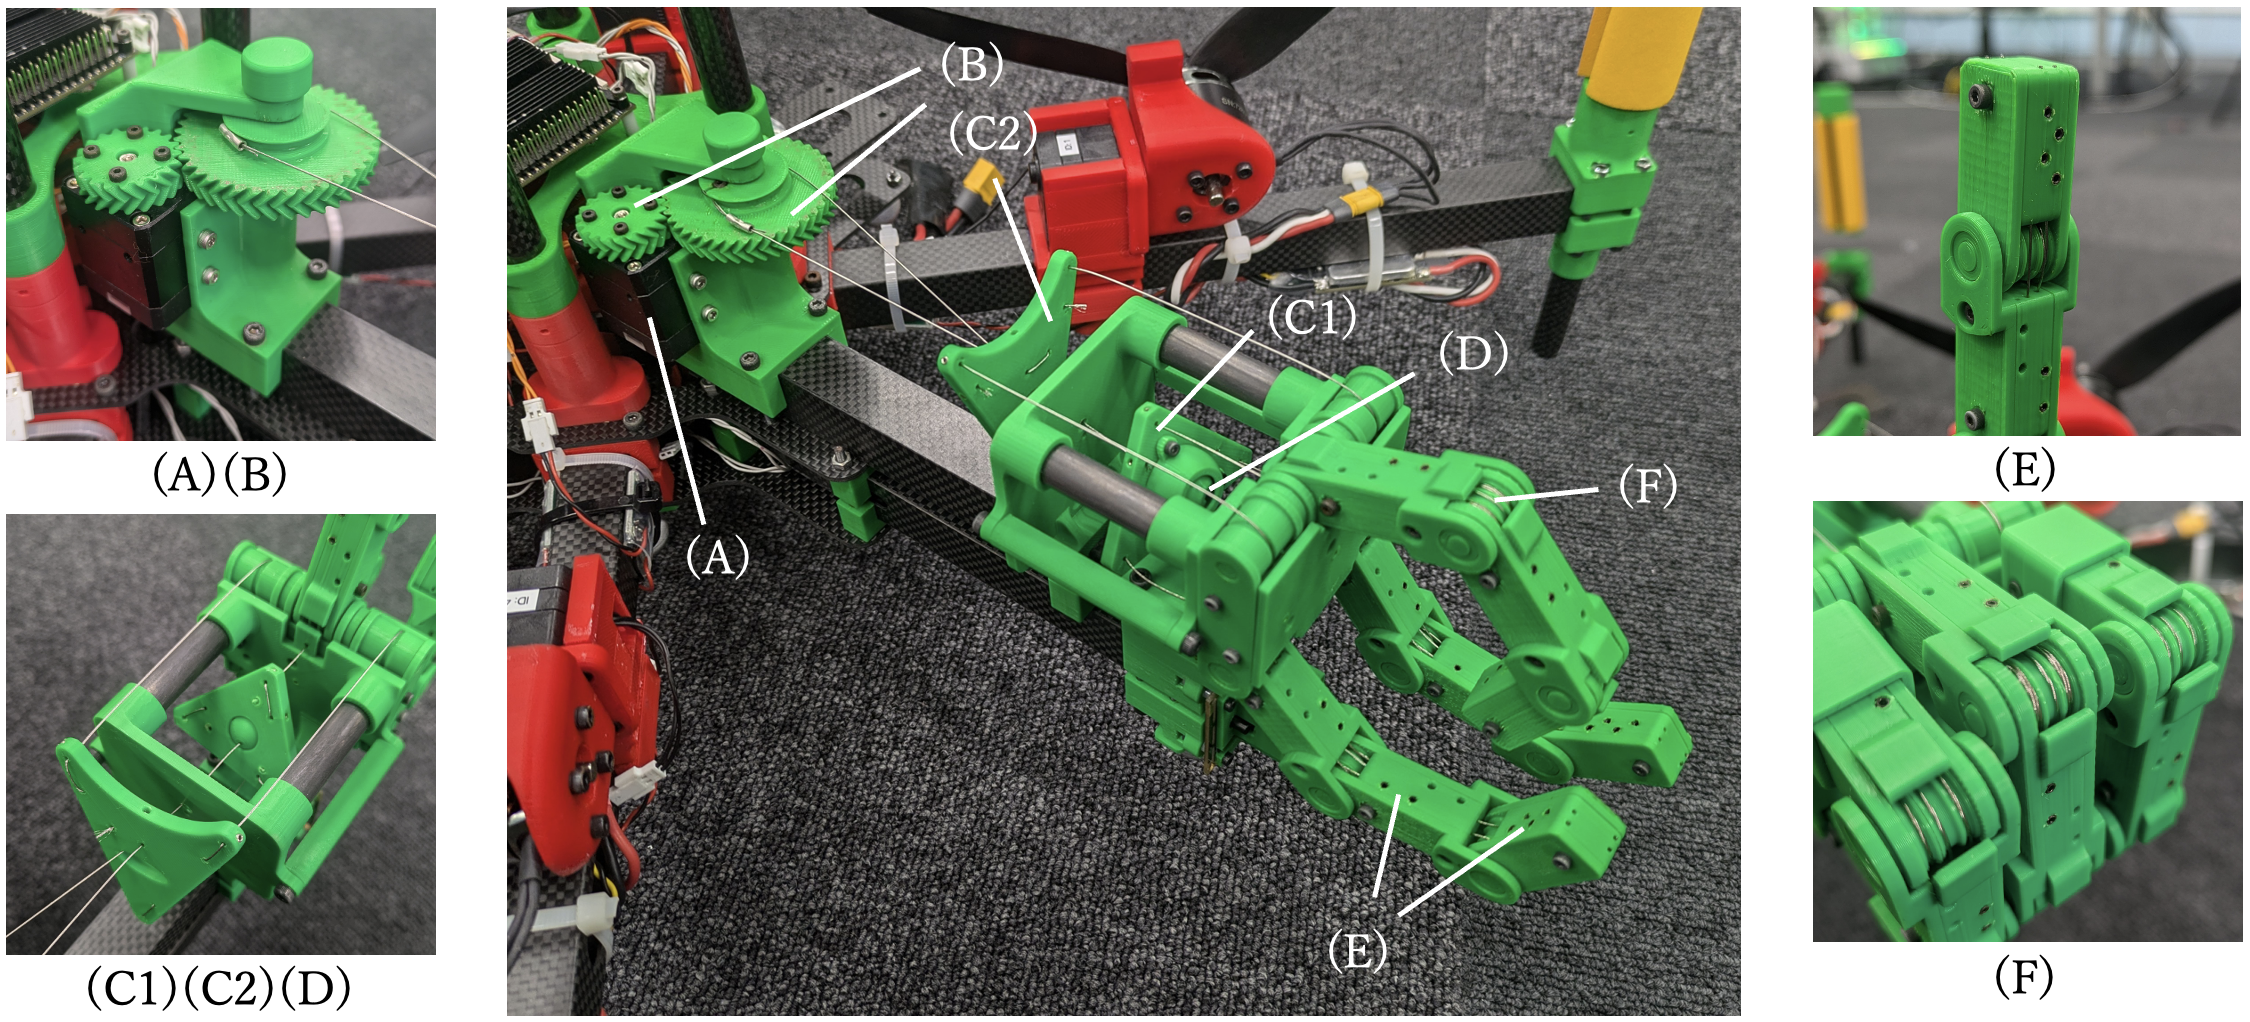
\includegraphics[width=0.8\columnwidth]{figs/zissou.eps}
  \caption{Hand detail}
  \vspace{-2mm}
  \label{fig:zissou}
\end{figure}
ハンドの実制作にあたり、軽量性を重視しPLA素材とCFRPパイプを用いた。アクチュエータとしてDynamixel XH350-W210Rを採用し、山歯歯車により2倍に減速した。またステンレスワイヤと止めねじにより各指内部に3層の腱構造を構築した。ハンド全体の重量はおよそ390gとなった。
\subsection{物体把持能力検証}
\vspace{-2mm}
\begin{figure}[h]
  \centering
  \includegraphics[width=0.8\columnwidth]{figs/grasping.eps}
  \caption{Grasping experiment with various shape objects}
  \vspace{-2mm}
  \label{fig:zissou}
\end{figure}
ハンドの把持能力を検証するため、8種類の形状に対して物体把持試験を行った。先行研究では不可能であったハンドの初期状態によらない多様な凹凸形状への従動的な把持に加えて、直径が大きく異なる物体や円柱、箱、薄板、球体および実際の電動工具のような複雑形状も把持可能であった。
\subsection{支持可能重量検証}
\begin{figure}[tb]
  \centering
  \begin{subfigure}{0.28\columnwidth}
    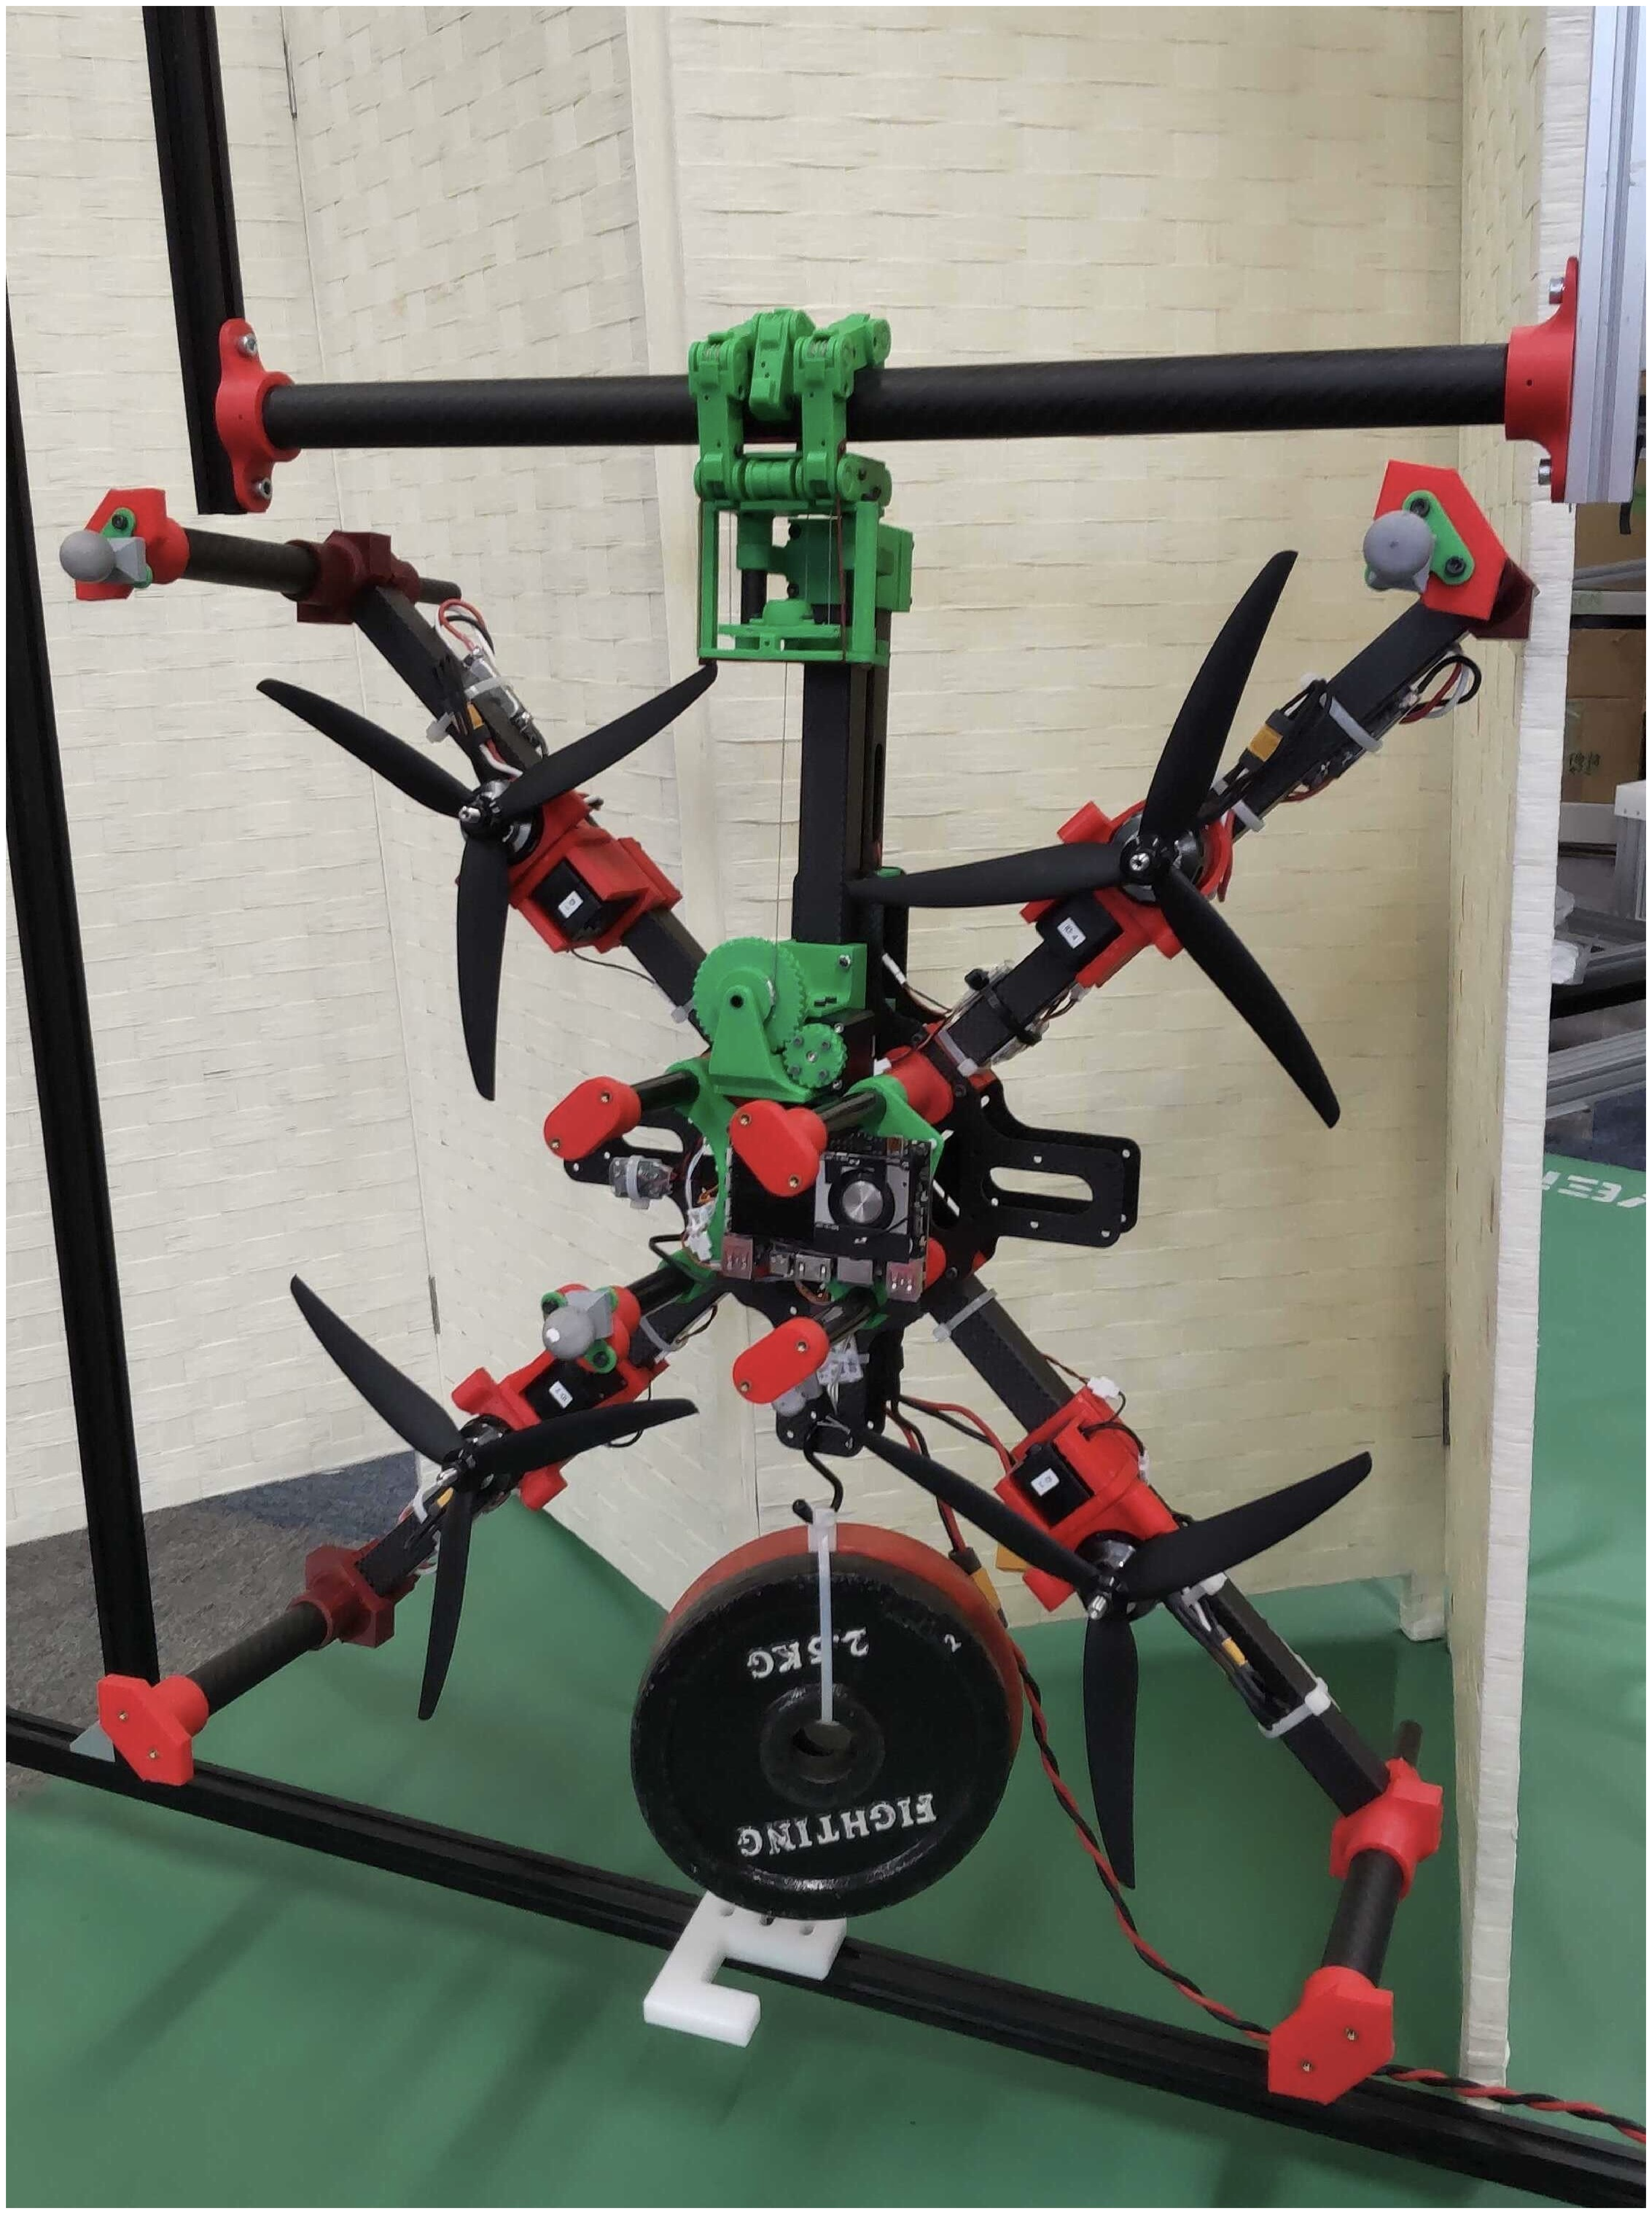
\includegraphics[width=\textwidth]{figs/bear1.eps}
    \vspace{-6mm}
    \caption{}
    \label{fig:bear1}
  \end{subfigure}
  \begin{subfigure}{0.6\columnwidth}
    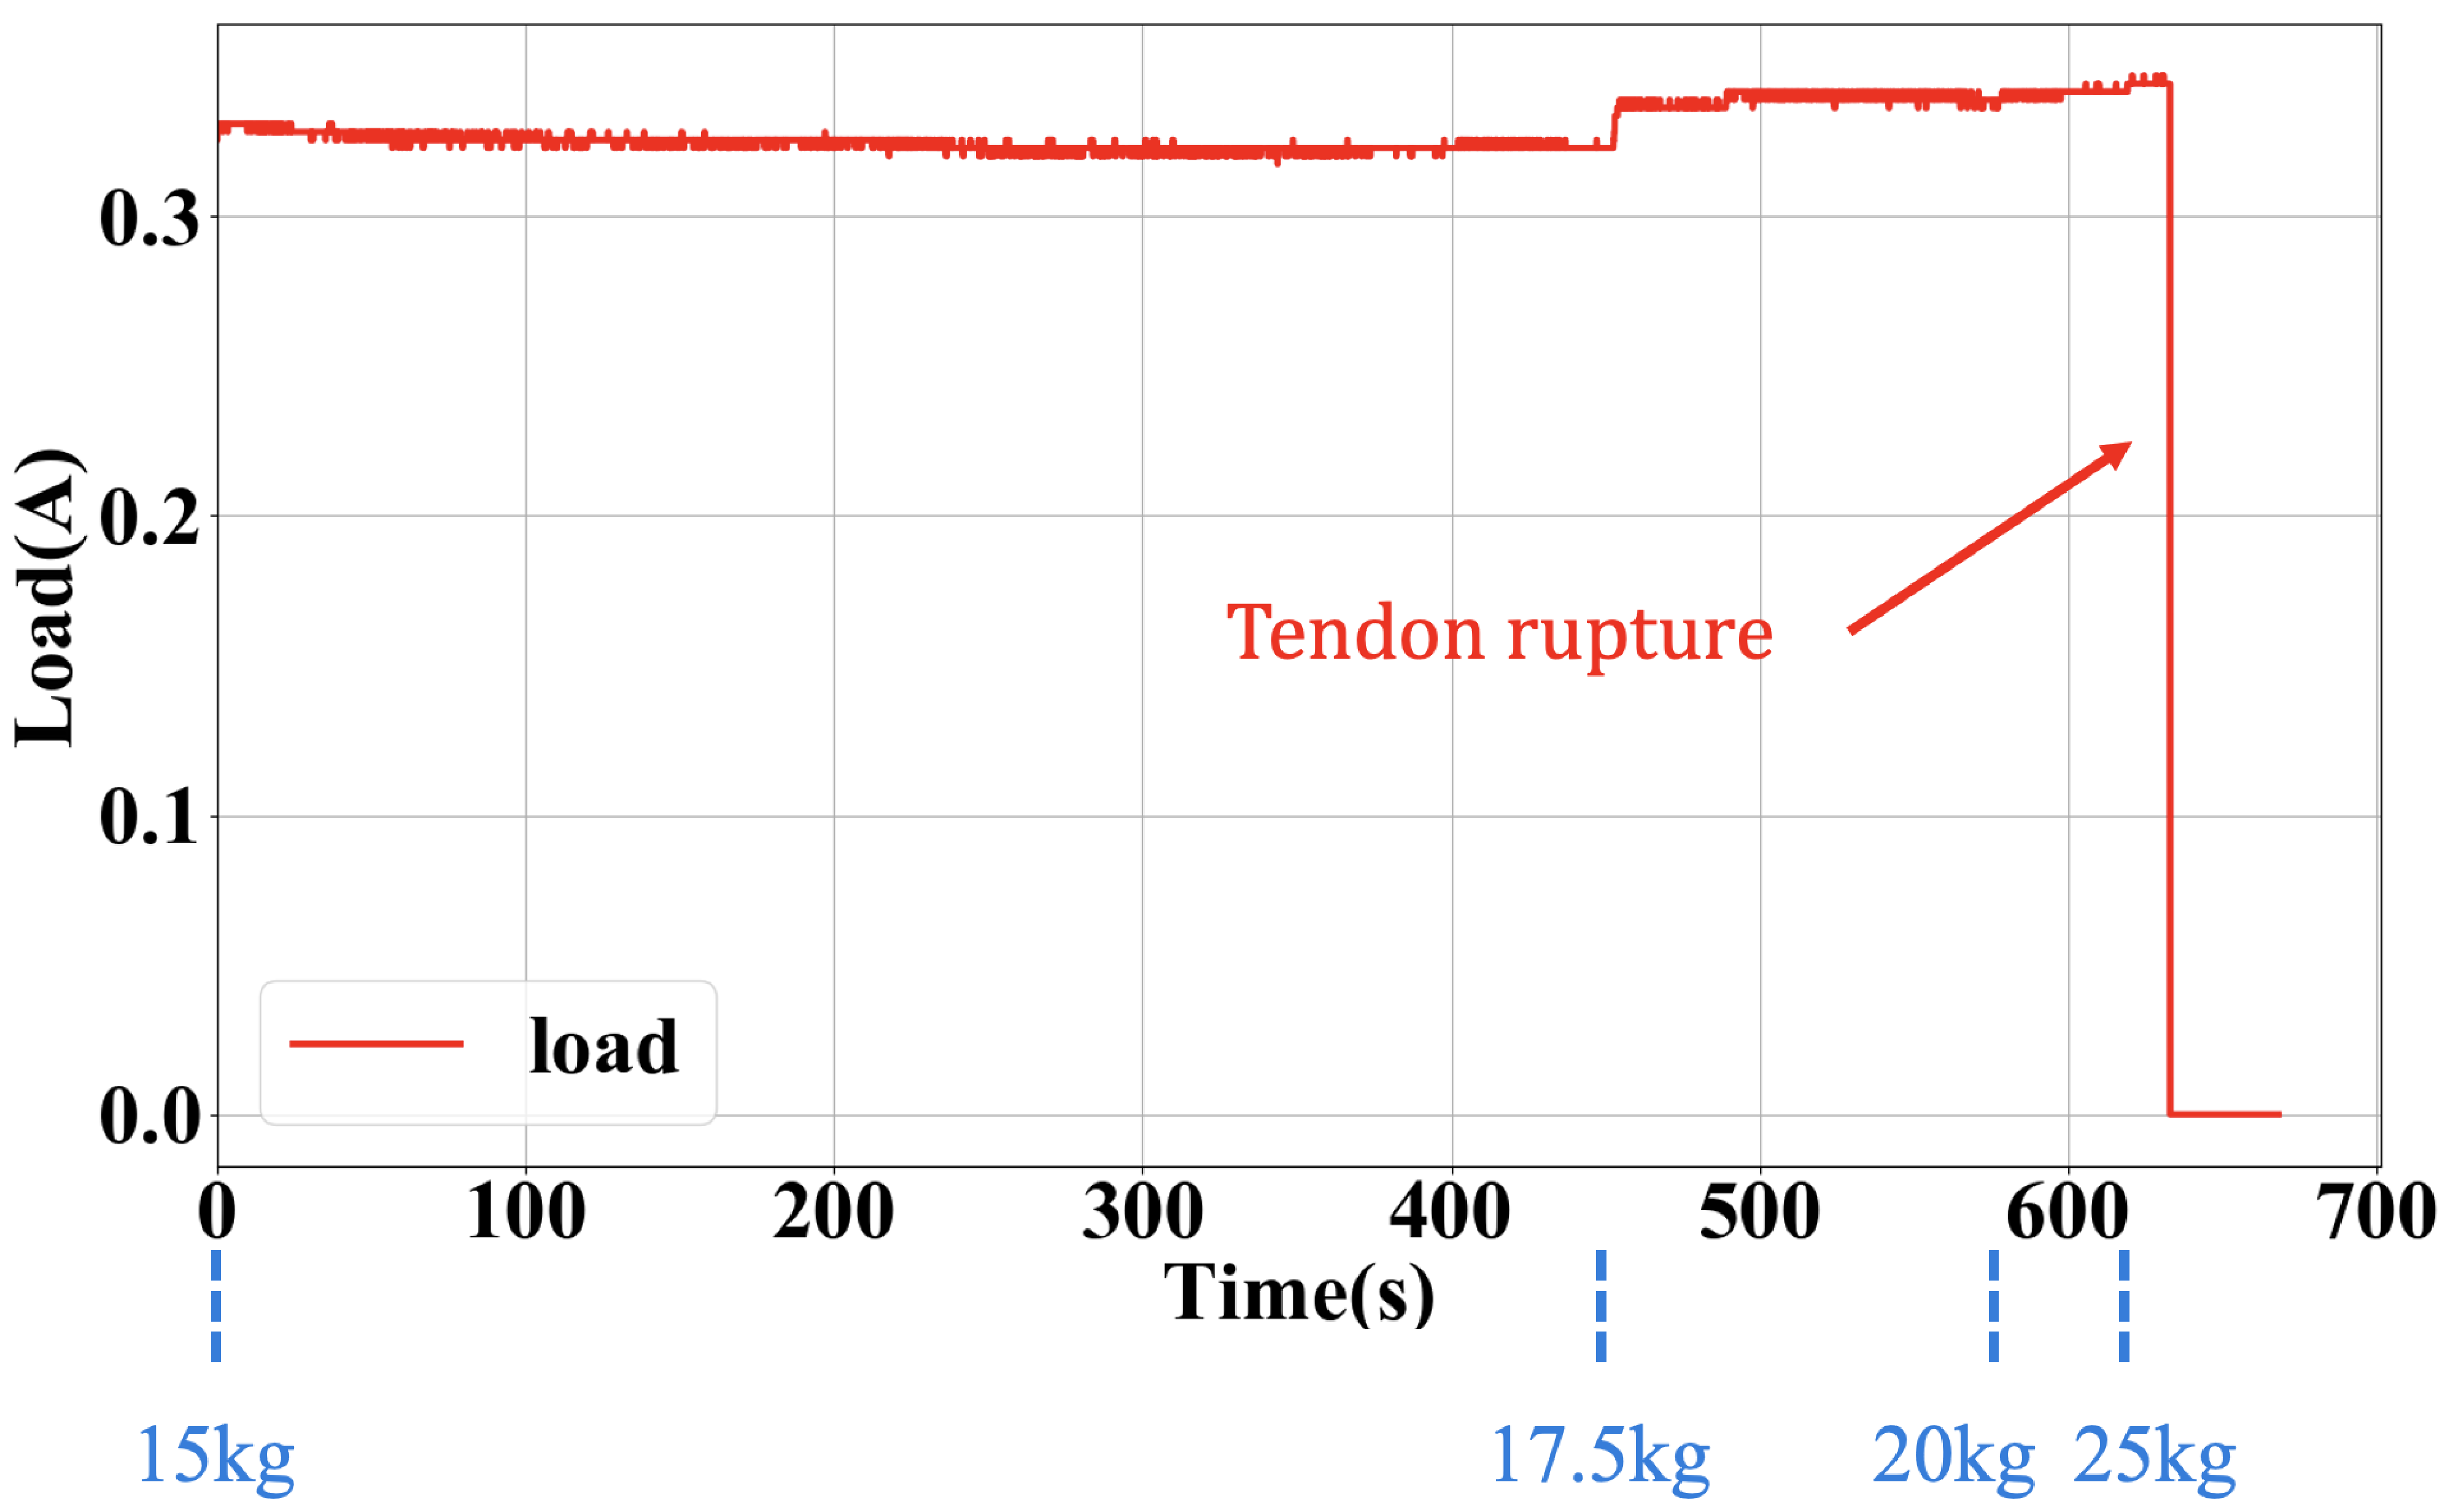
\includegraphics[width=\textwidth]{figs/bear2.eps}
    \vspace{-6mm}
    \caption{}
    \label{fig:bear2}
  \end{subfigure}
  \vspace{1mm}
  \caption{Perching and grasping image}
  \vspace{-4mm}
\end{figure}
図\ref{fig:bear1}に示すように、直径24mmのCFRPパイプにハンドを結合させ、機体に2.5kgずつ重量を付加した。また式\ref{equ:mmaxb}から、制作したハンドが支持可能な最大重量は29.6kgと算出されたが、結果として機体自重の約11倍である27.5kgに達した時点で主腱の破断が生じた。実験後に致命的な指構造の破壊はみられなかったため、主腱の引張強度不足が原因であると考えられる。図\ref{fig:bear2}は腱破断までのサーボ負荷のプロットである。プロットからサーボ負荷は全体を通して平坦であるが、17.5kgを付加したt=450s付近で小さな段差が見られる。この時点においてハンドが図\ref{fig:weight2}の状態へ移行する様子が観察されたため、第2章で述べた支持可能重量の急激なジャンプによりサーボ負荷が一時的に上昇したものと考えられる。この結果から、トライフォース・ハンドは自重に対して十分に大きな重量を支持可能であることが示された。
\subsection{ペンデュラム・パーチングおよび離陸検証}
\vspace{-2mm}
\begin{figure}[h]
  \centering
  \begin{subfigure}{0.38\columnwidth}
    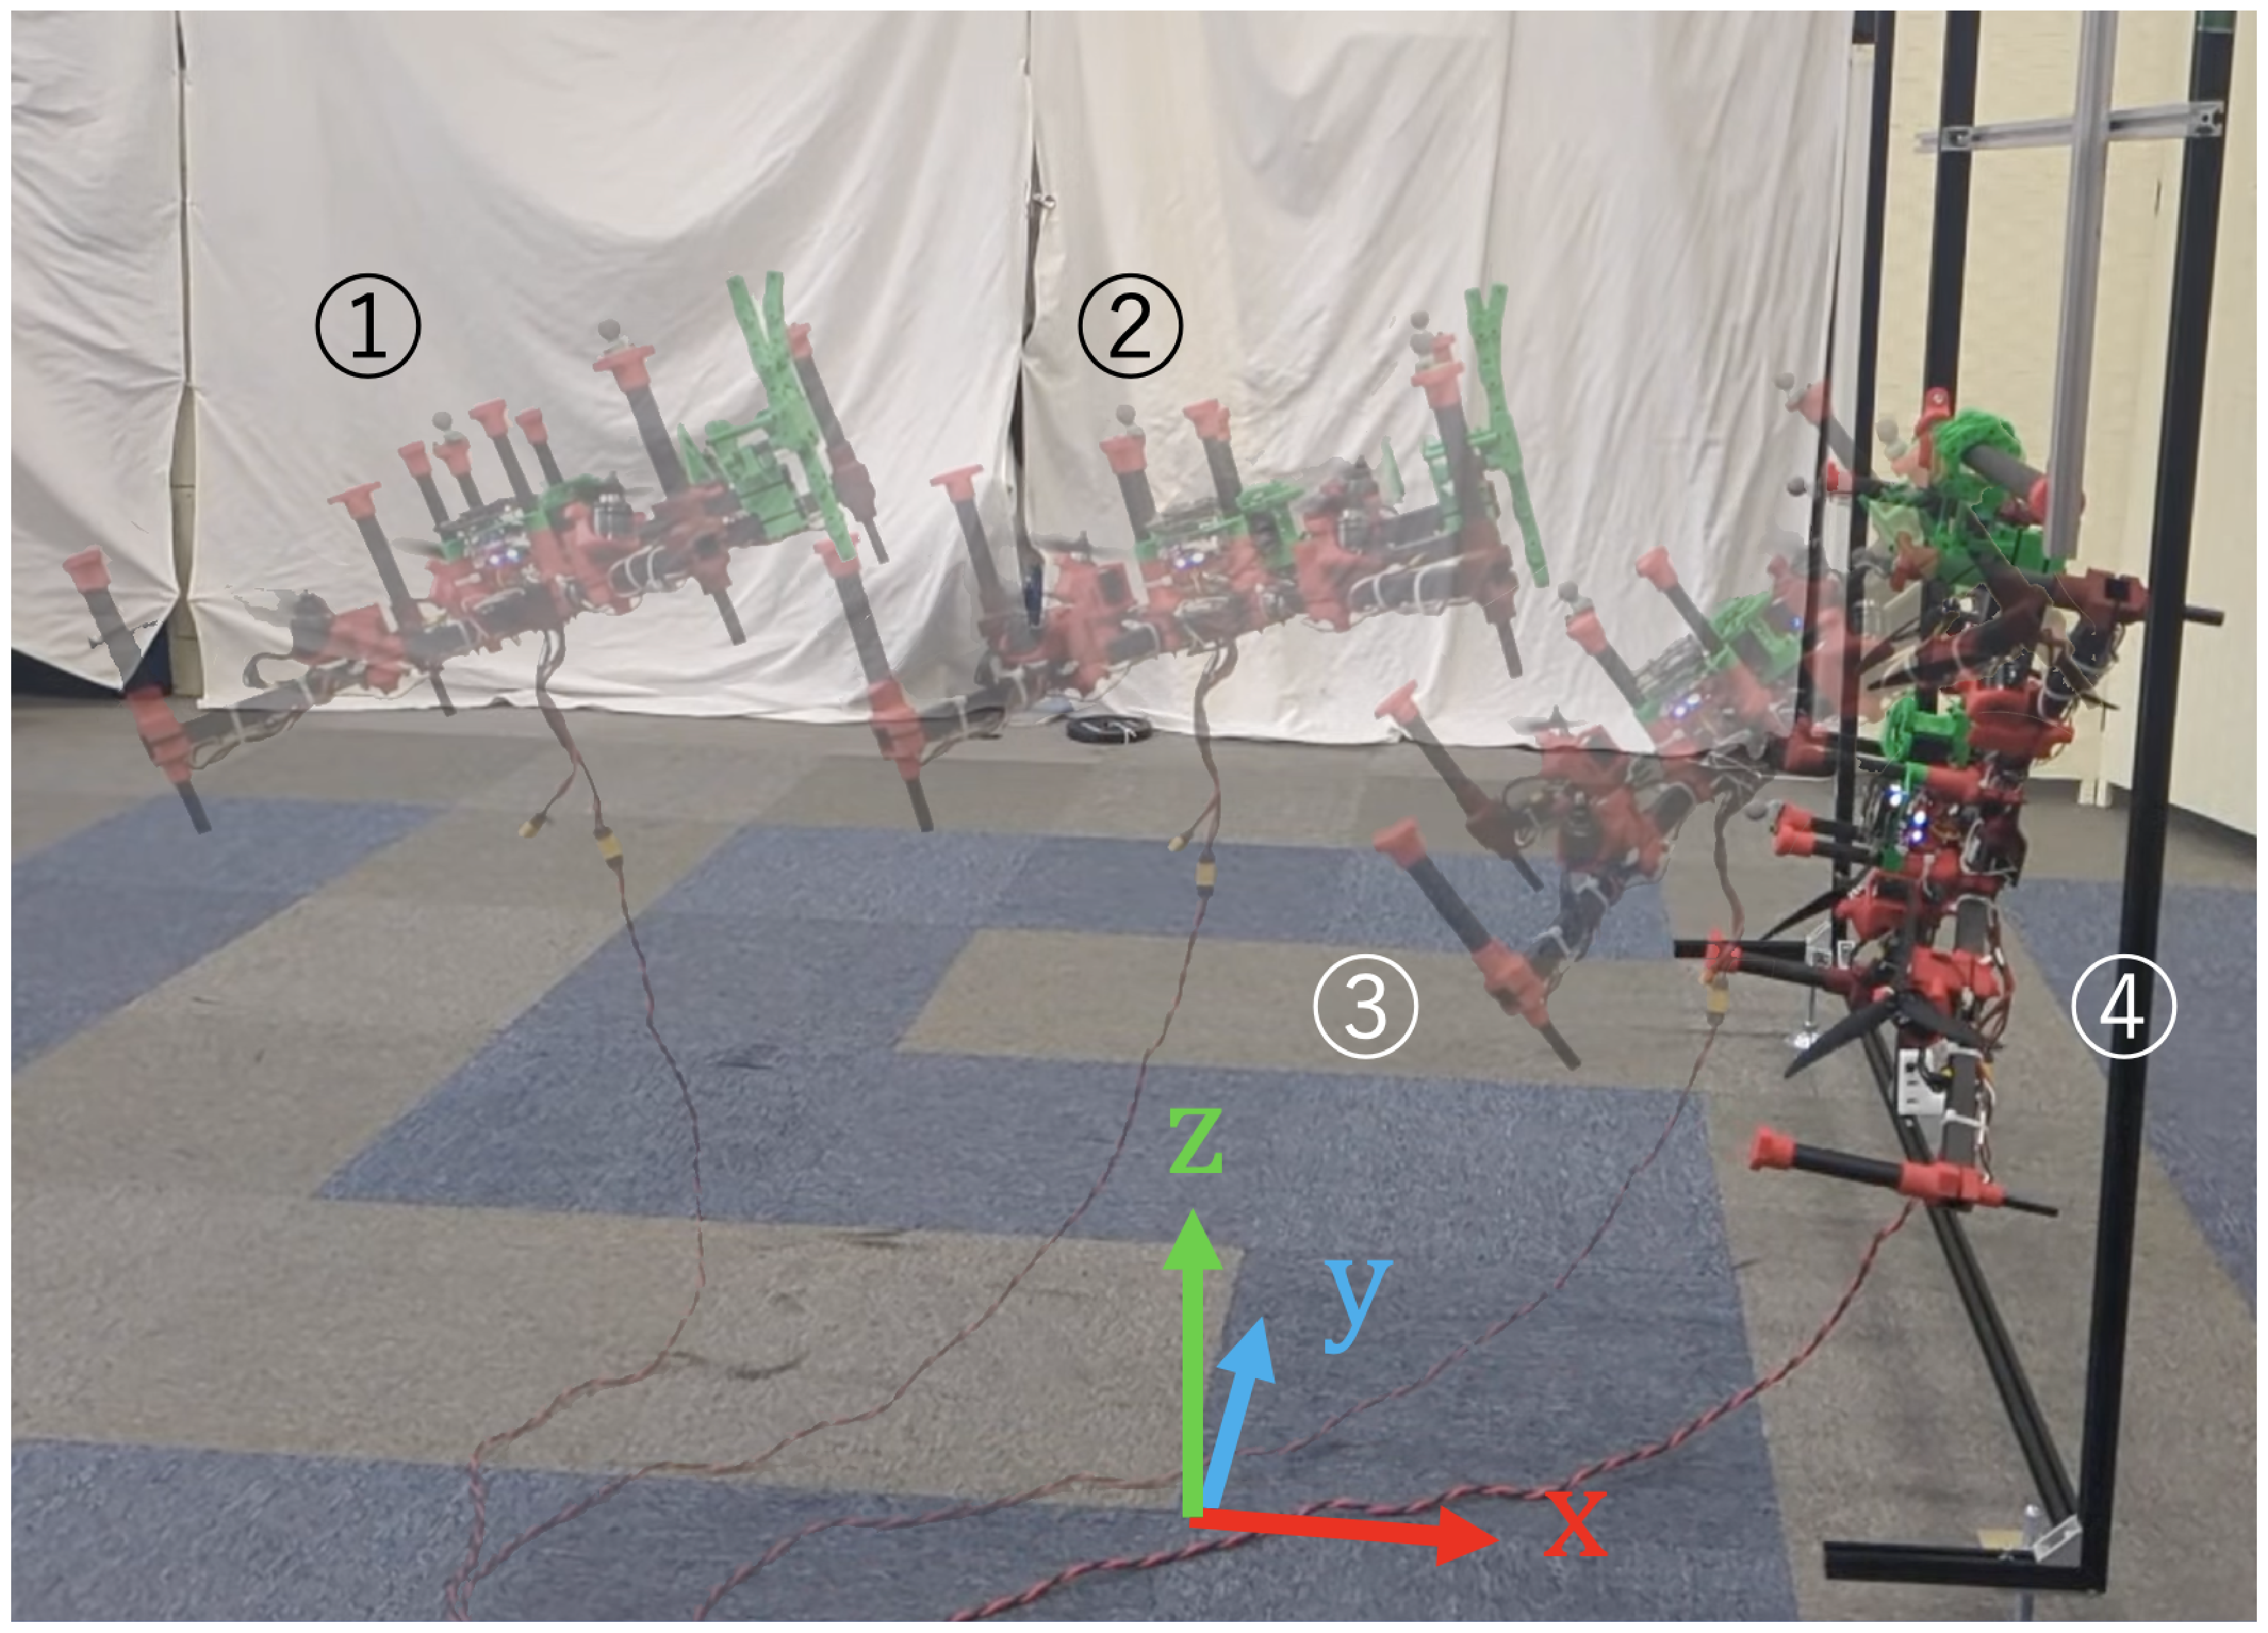
\includegraphics[width=\textwidth]{figs/attaching.eps}
    \vspace{-6mm}
    \caption{}
    \label{fig:perching1}
  \end{subfigure}
  \begin{subfigure}{0.38\columnwidth}
    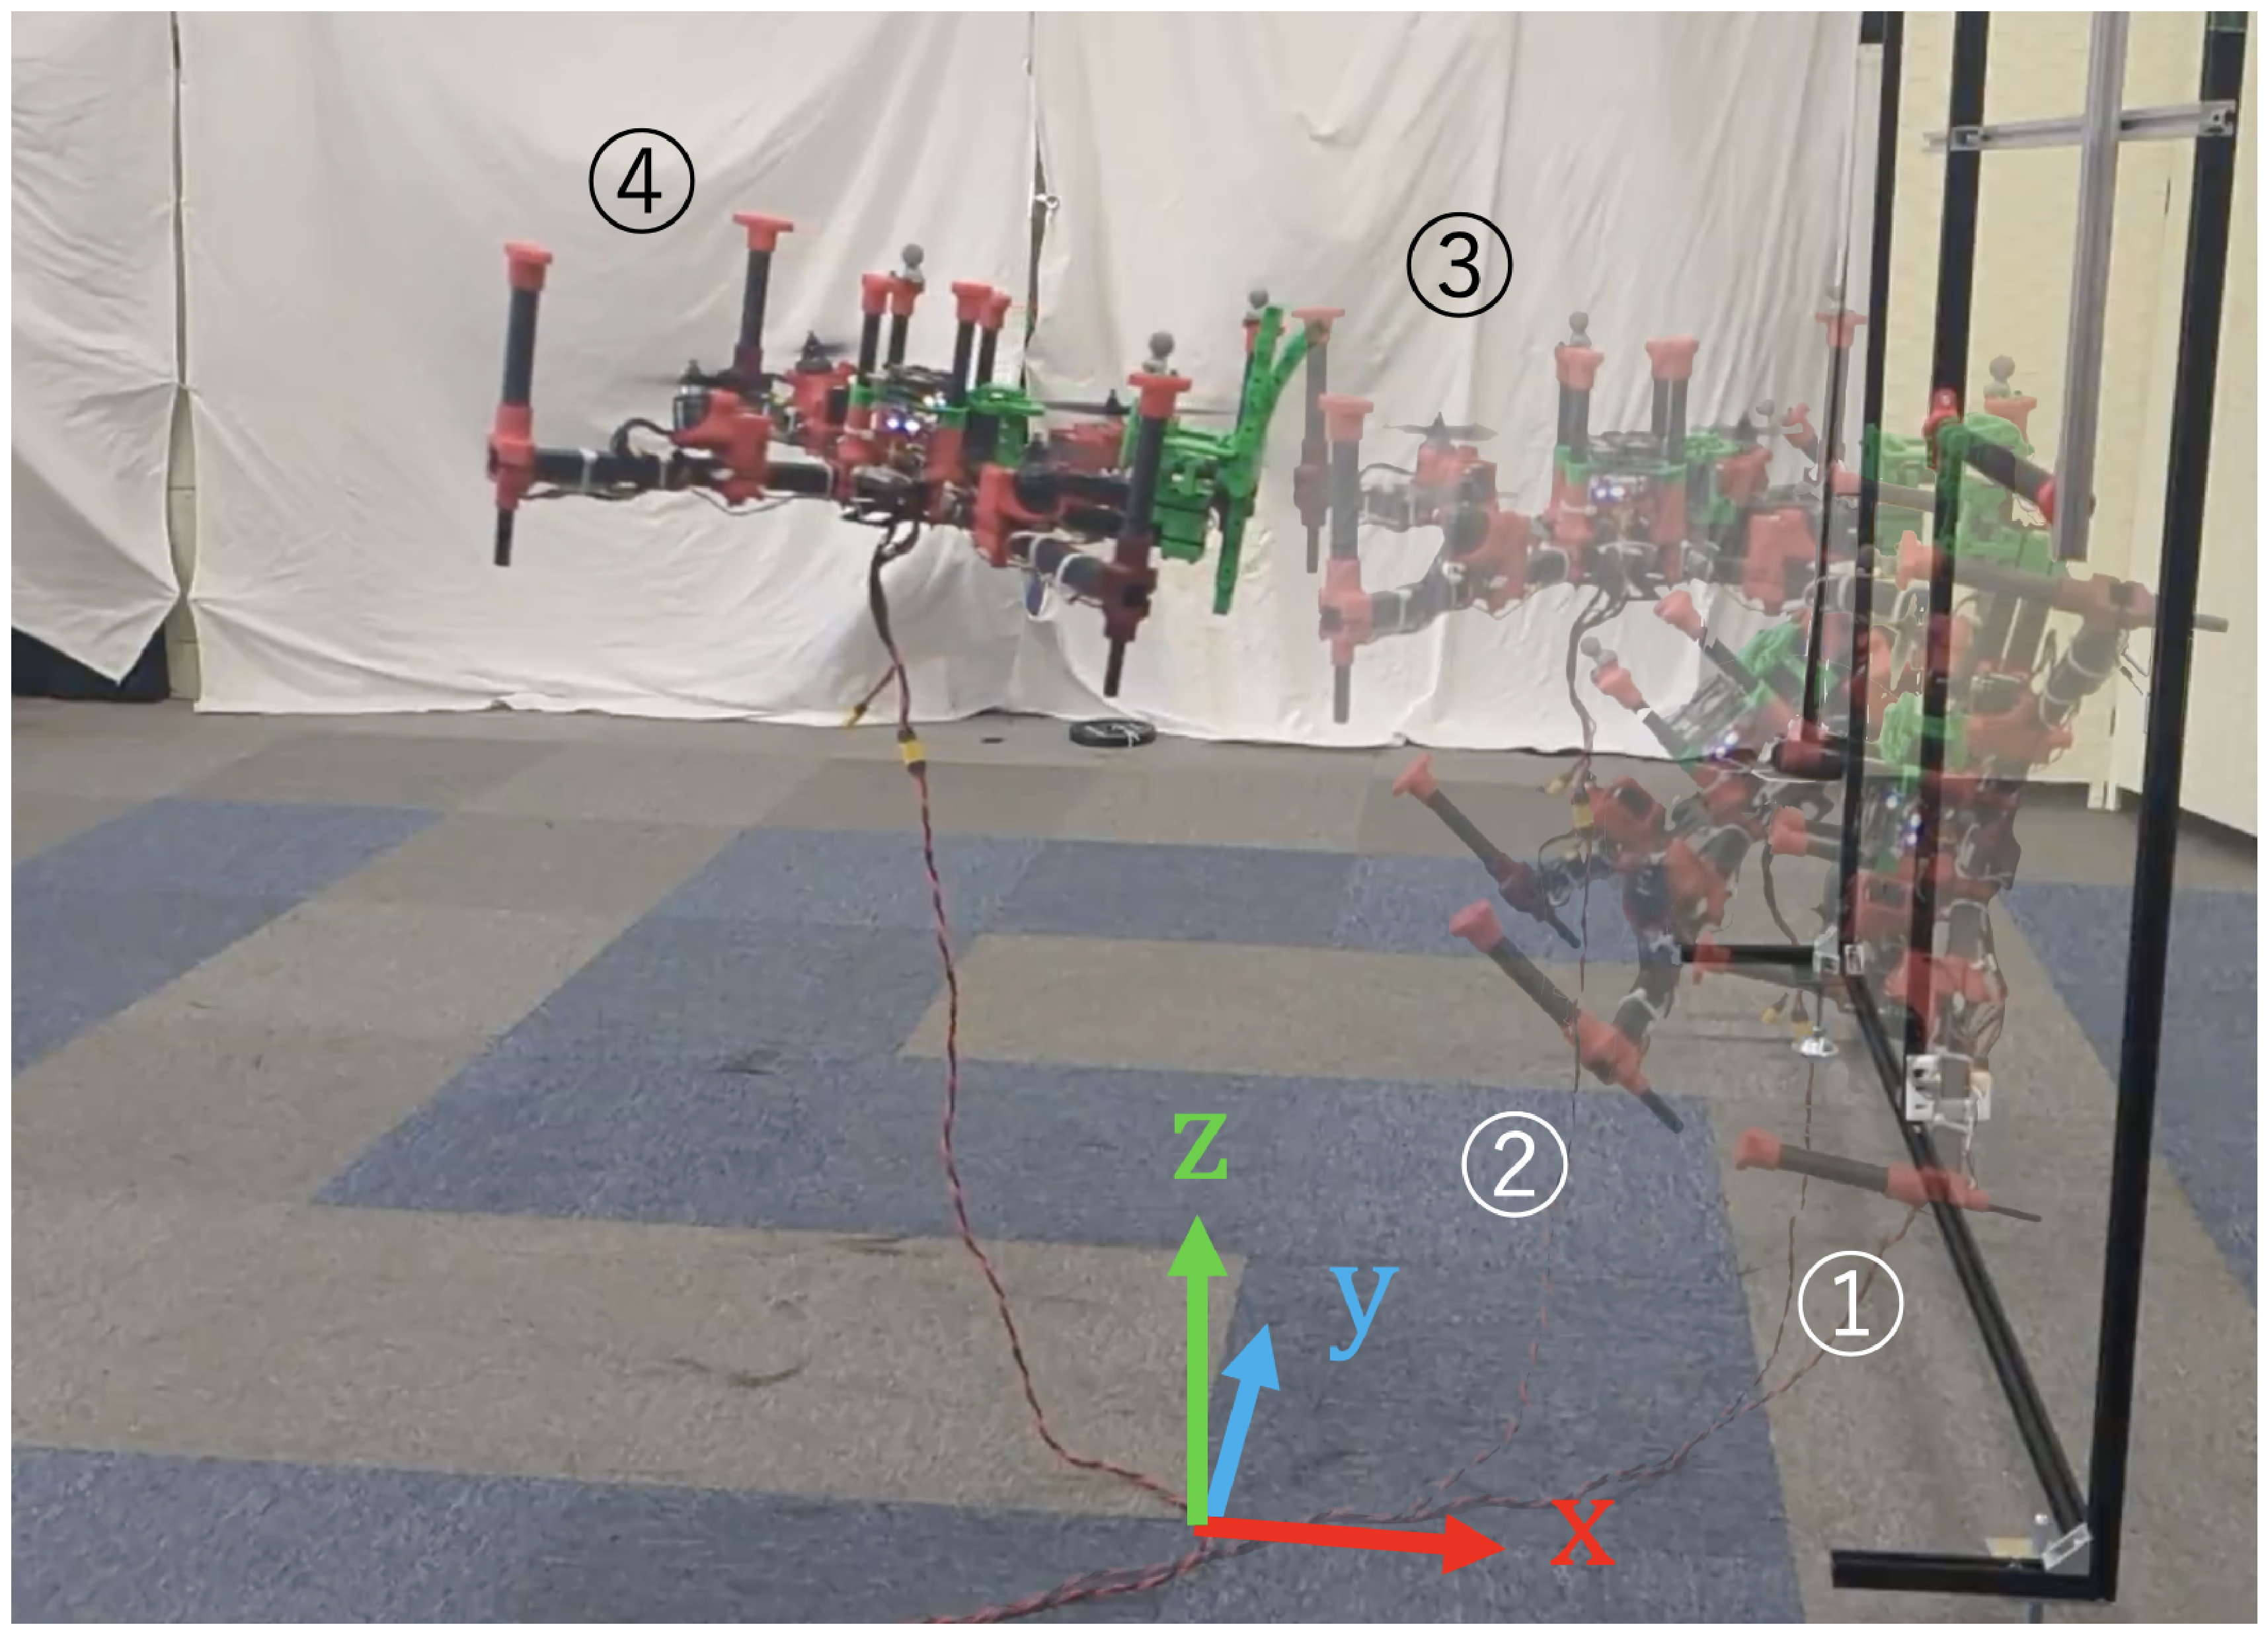
\includegraphics[width=\textwidth]{figs/detaching.eps}
    \vspace{-6mm}
    \caption{}
    \label{fig:perching2}
  \end{subfigure}
  \vspace{1mm}
  \caption{Perching experiment}
  \label{fig:perching}
  \vspace{-4mm}
\end{figure}
\vspace{-2mm}
\begin{figure}[h]
  \centering
  \begin{subfigure}{0.38\columnwidth}
    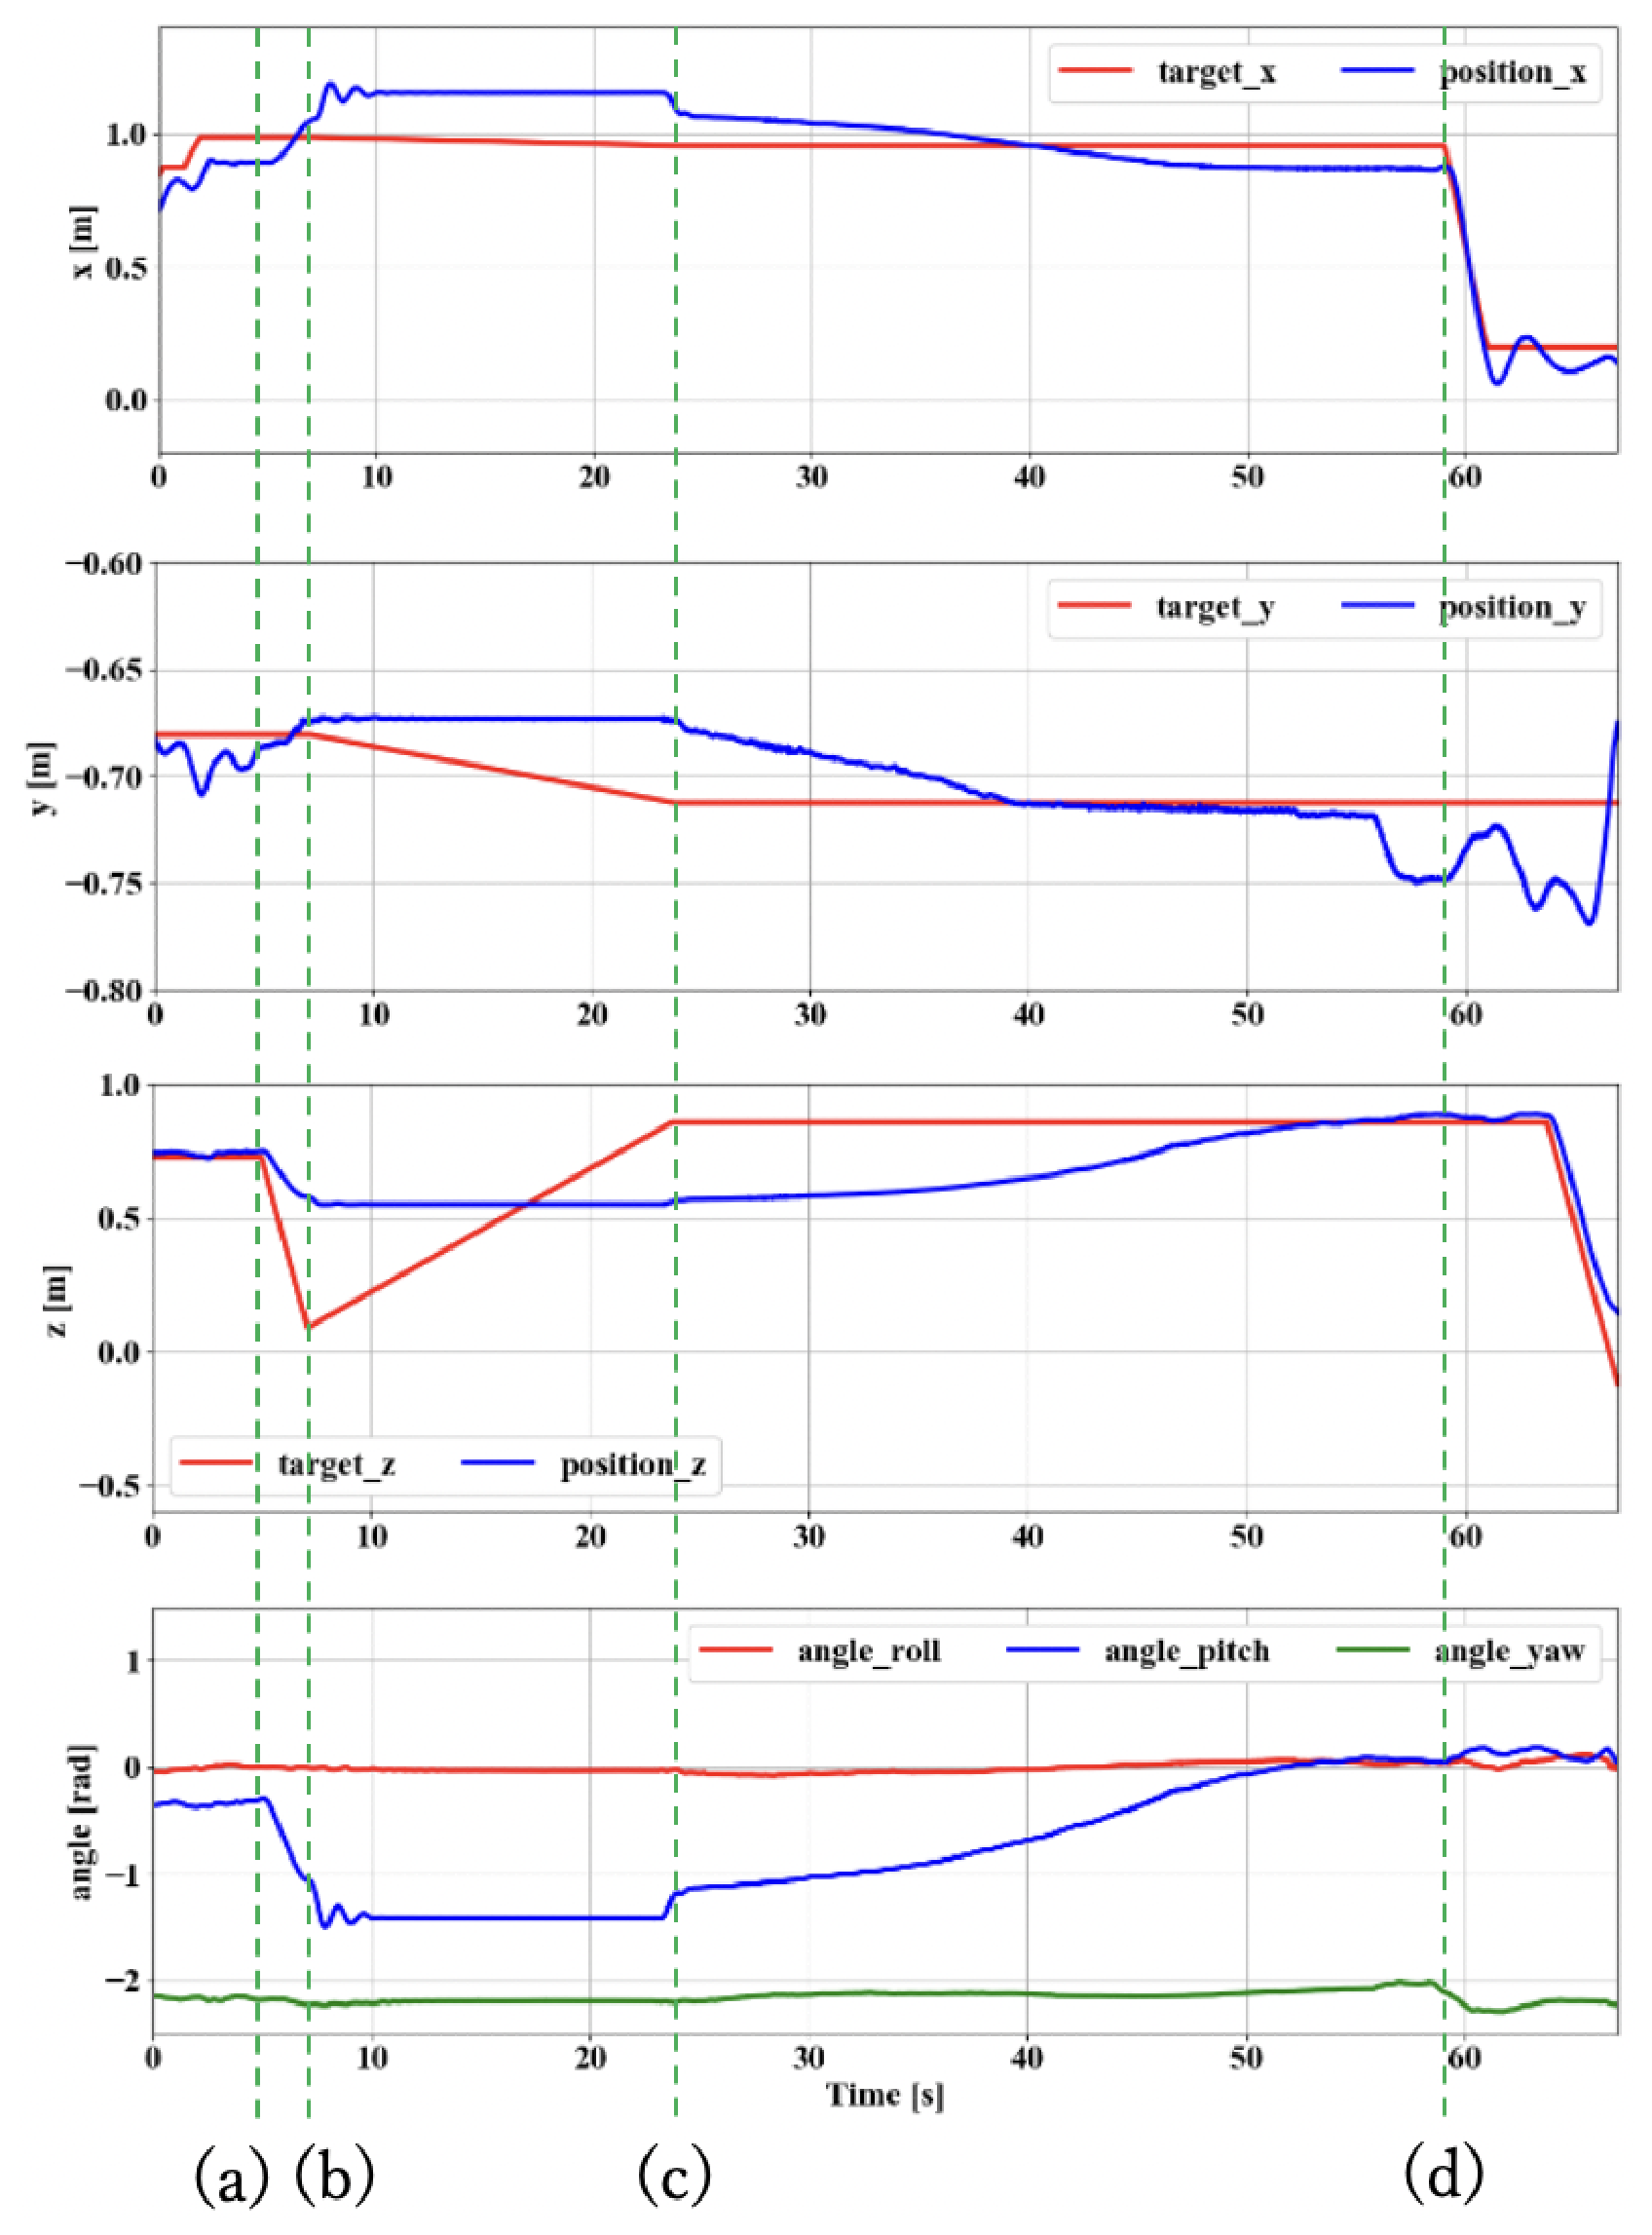
\includegraphics[width=\textwidth]{figs/plot1.eps}
    \vspace{-6mm}
    \caption{}
    \label{fig:plot1}
  \end{subfigure}
  \begin{subfigure}{0.38\columnwidth}
    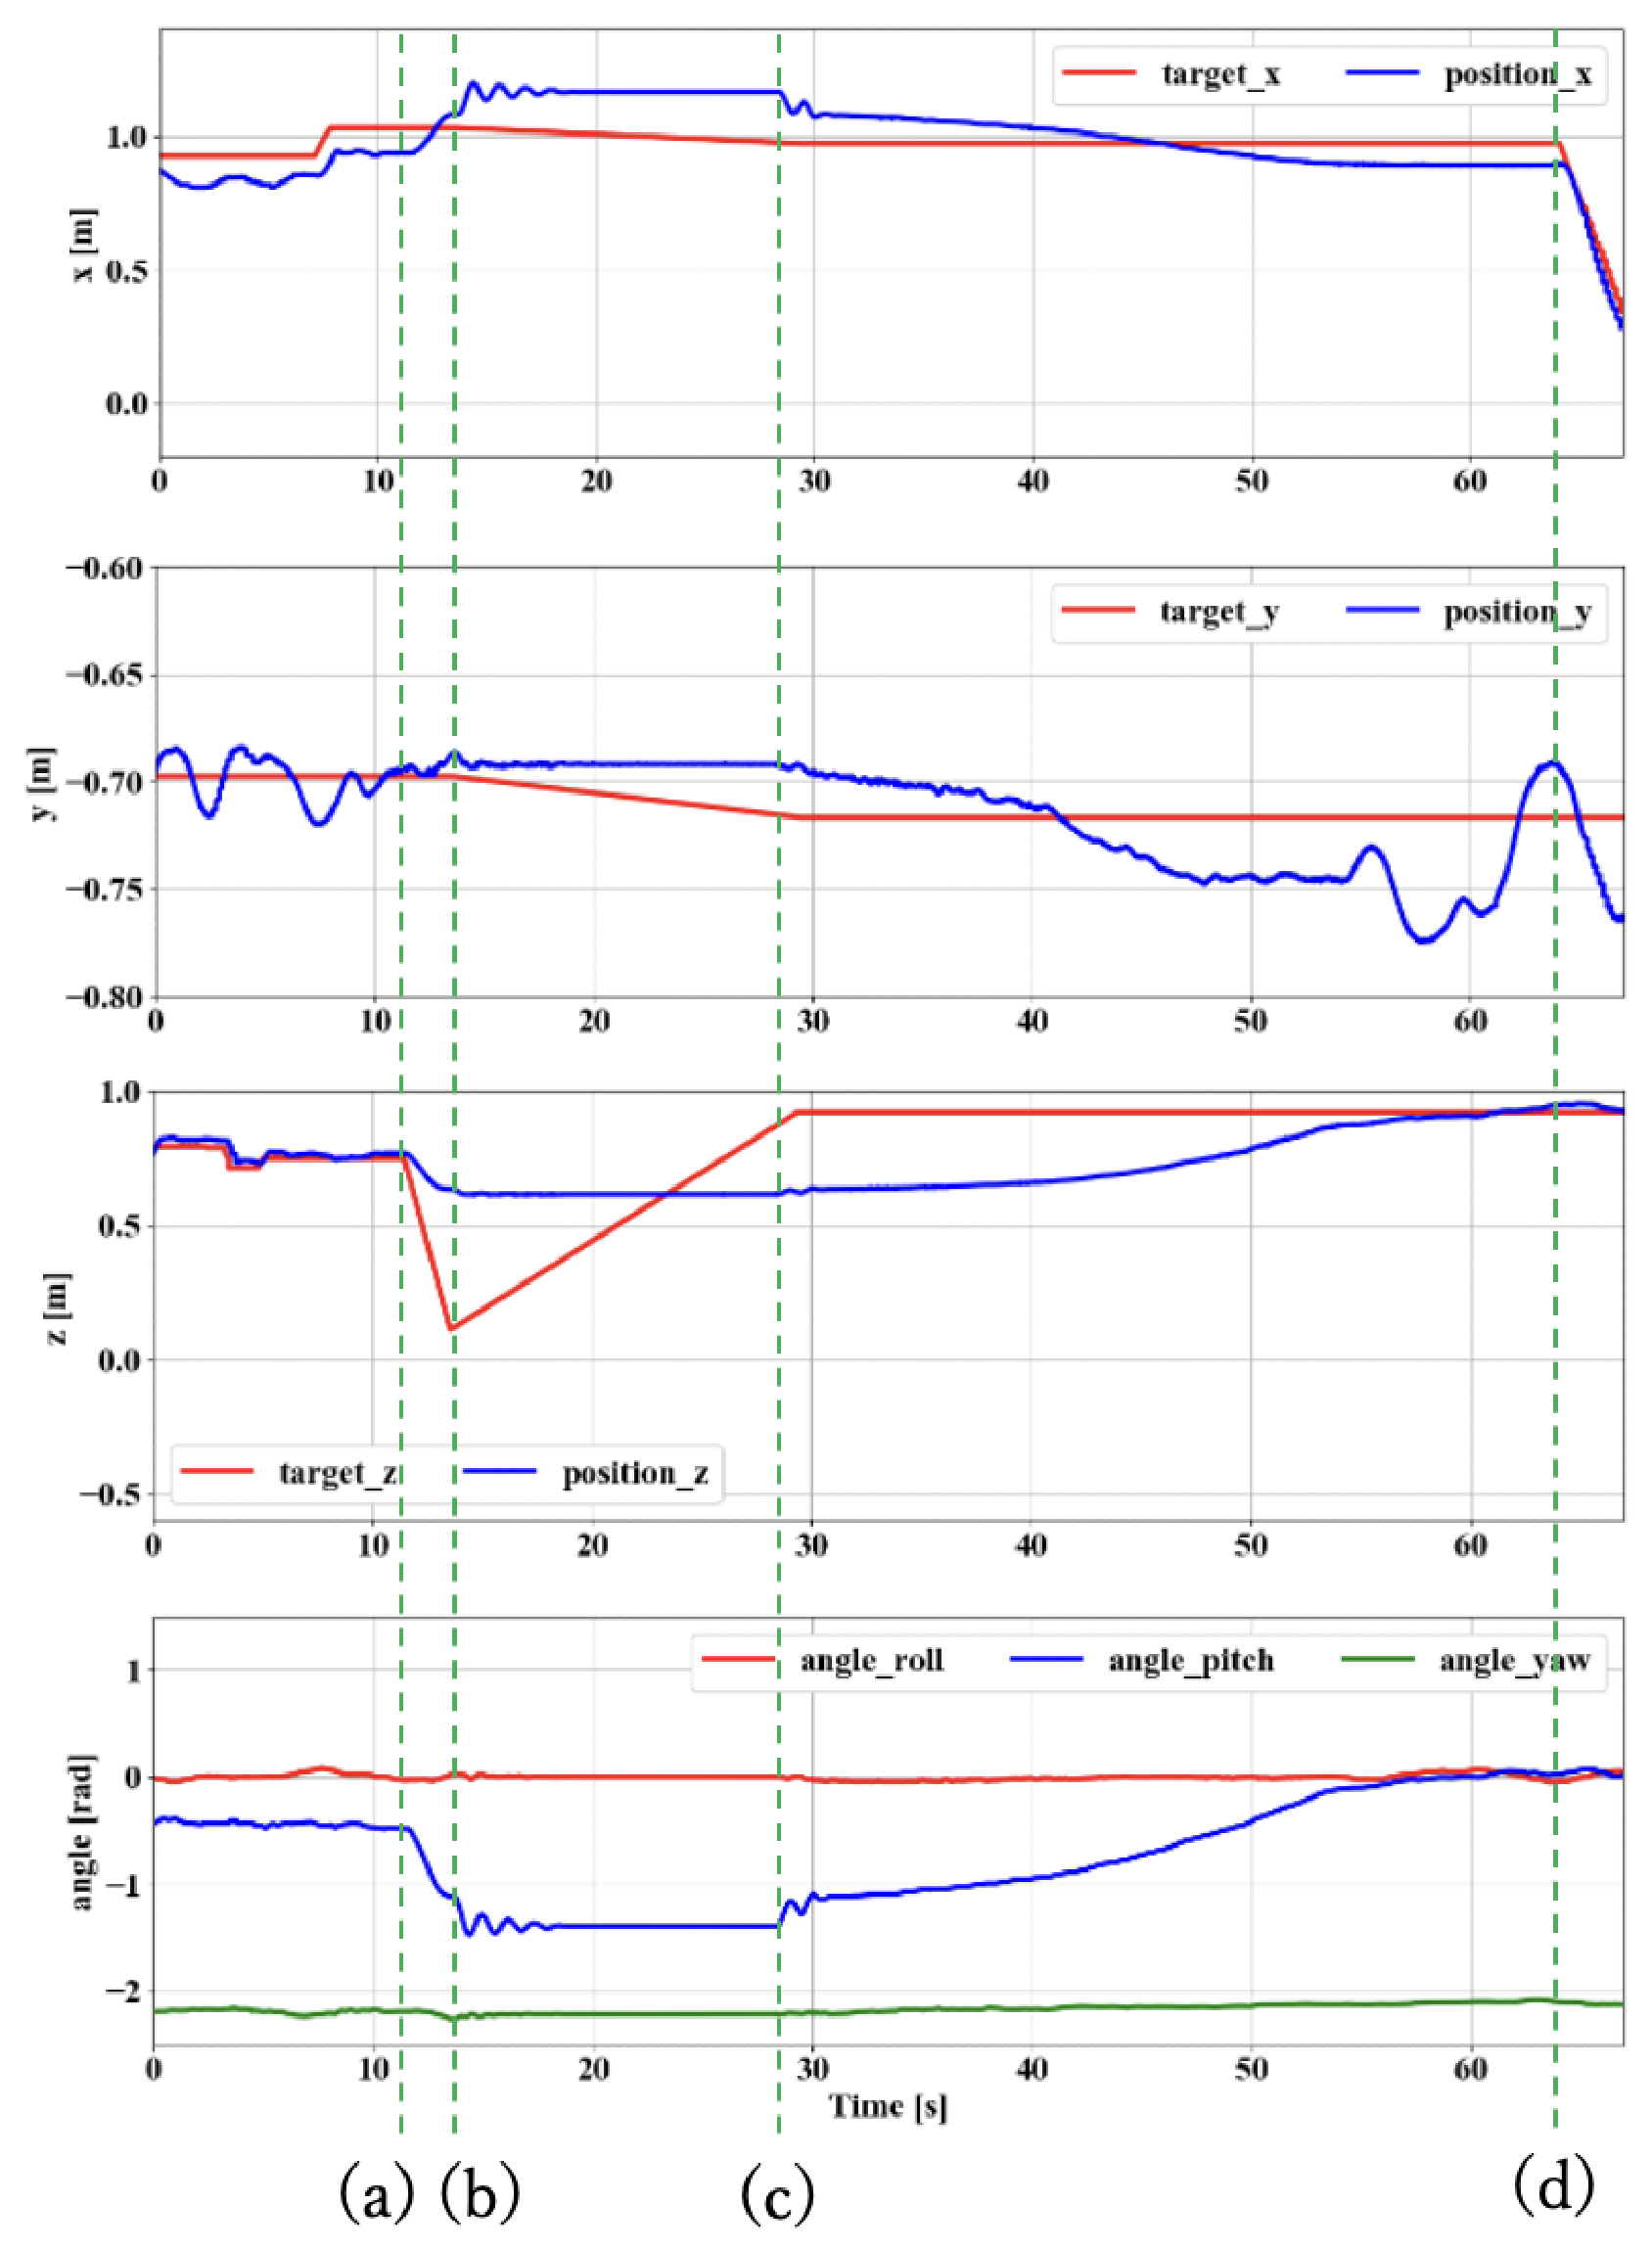
\includegraphics[width=\textwidth]{figs/plot2.eps}
    \vspace{-6mm}
    \caption{}
    \label{fig:plot2}
  \end{subfigure}
  \vspace{1mm}
  \caption{Plots of position and angle during perching}
  \label{fig:plot}
  \vspace{-2mm}
\end{figure}
提案した機体構成によるパーチングの検証試験として、図\ref{fig:bear1}の実験装置を用い、直径24mmの円柱および20mm四方の角柱への結合/解離試験を行った。姿勢制御には第3章で述べた動作計画を用いた。図\ref{fig:perching}に円柱への結合・解離実験時の様子を示す。また、図\ref{fig:plot1}に円柱へのパーチングアプローチから解離までの機体位置と目標位置の誤差、および機体角度のプロットを示す。

プロットから、離陸過程において機体位置が正しく目標位置に収束していることが読み取れる。また積分要素の再計算により、解離直後のx方向における目標位置の大きな変化にも追従できている。y座標に見られる5cm前後の誤差は、各指モジュールが同時に開閉しないことにより解離時の結合抵抗が左右で均一とならず、機体が左右に振れたことが原因であると考えられる。

図\ref{fig:plot2}は角柱への結合/解離試験における機体位置と角度のプロットである。円柱とは異なり、角柱へのペンデュラム・パーチングの実行においては結合物体の直径が機体の回転に伴って変化する。従って強く把持した状態で着陸動作を行った場合、指を開く方向への力によってサーボモータに強い負荷が生じ、オーバーロードに繋がる可能性がある。この問題への対処として、結合時にハンドの握りを意図的に緩めることでサーボモータのオーバーロードを防ぎつつ角柱へのパーチングと解離を実現した。角柱の縁と指関節の小さな抵抗により、図\ref{fig:plot2}のt=29s付近などに図\ref{fig:plot1}にはみられない揺らぎが観察されたが、振れの大きさは十分に小さく、該当部分の前後においても滑らかな動作が継続可能であった。結果として、トライフォース・ハンドおよび提案した動作計画を用いたペンデュラム・パーチングの実現可能性が示された。

\section{結論と今後の展望}

\footnotesize
% \begin{thebibliography}{99}
\bibliographystyle{junsrt}
\bibliography{bib.bib}
% \bibitem{Shinjuku98}
% 新宿大五朗,渋谷次郎,東京 学,``キャスティングマニピュレーションに関する研究(第1報,可変長の紐状柔軟リンクを有するマニピュレータの提案とそのスイング制御法)'',{\it 機論C編}, vol.64-626, pp.3854--3861, 1998.

% \bibitem{Shinjuku99}
% Shinjuku, D., Shibuya, J. and Tokyo, M., ``Swing Motion Control of Casting Manipulation,'' {\it IEEE Control Systems}, vol.19-4, pp.56--64, 1999.

% \end{thebibliography}

\normalsize
\end{document}
